\documentclass[11pt]{article}

% remember to put in something from that paper with the diagram about
%difference annulling vows when under the authority of a father and husband
%  sudo apt-get install culmus
%  sudo apt-get install texlive-xetex
%  sudo apt-get install texlive-latex-extra
%  sudo apt-get install texlive-lang-hebrew
%  sudo apt-get install texlive-lang-other texlive-lang-arabic
%  sudo apt-get install texlive-fonts-extra texlive-latex-extra


\makeatletter
\def\Year#1{%
  \def\yy@##1##2##3##4;{##1##2##3##4}%
  \expandafter\yy@#1;
}
\makeatother


\usepackage[utf8]{inputenc}
\usepackage{titlesec}
\usepackage{lipsum}
\usepackage{listings}
\lstset{
  columns=fullflexible,
  frame=single,
  breaklines=true
}

\setcounter{secnumdepth}{4}
\titleformat{\paragraph}
{\normalfont\normalsize\bfseries}{\theparagraph}{1em}{}
\titlespacing*{\paragraph}
{0pt}{3.25ex plus 1ex minus .2ex}{1.5ex plus .2ex}

\usepackage{graphicx}
\graphicspath{ {images/} }


\makeatother
\usepackage[hyphens]{url}

\usepackage{polyglossia}
\setdefaultlanguage{english}
\setotherlanguage{hebrew}
\setotherlanguage[variant=ancient]{greek}
\usepackage{fontspec}
\newfontfamily\greekfont[Script=Greek]{Linux Libertine O}


%linux settings
\setmonofont{Miriam Mono CLM}
\setsansfont{Simple CLM}
\setmainfont{Frank Ruehl CLM}


%windows settings
%\setmainfont{Arial}
% to change font for Hebrew
%\newfontfamily\hebrewfonttt[Script=Hebrew]{Miriam Mono CLM}
%\newfontfamily\hebrewfontsf[Script=Hebrew]{Simple CLM}
%\newfontfamily\hebrewfont[Script=Hebrew]{David CLM}

\usepackage{datetime2}

\usepackage[backend=biber]{biblatex}
\bibliography{\jobname}
\begin{filecontents}{\jobname.bib}
  @book{lit1,
    author      =   {Author, A. N.},
    title       =   {Title},
    publisher   =   {Publisher},
    address     =   {Location},
    year        =   {1066}}
\end{filecontents}

%makeatletter

\DeclareCiteCommand{\textcite}
  {\iffootnote{\usebibmacro{cite:init}}{}%
   \usebibmacro{prenote}}%
  {\usebibmacro{citeindex}%
   \iffootnote
     {\global\booltrue{cbx@mlafootnotes}%
      \renewcommand*{\newunitpunct}{\addcomma\space}%
      \usebibmacro{cite:mla:foot}}
     {\usebibmacro{cite:mla}}}
  {}
  {\usebibmacro{mla:foot:postnote}}

\makeatother

\bibliography{biblatex-examples}

\newcommand{\cmd}[1]{\texttt{\textbackslash #1}}
\setlength{\parindent}{0pt}




\title{\textbf{Deuteronomy 22:28-29} \large \\ Does the Torah punish rape? (rough draft) }
\begin{large}

\end{large}
\author{\textcircled{c} 2018-\the\year
 \ Anonymous \\ GNU Free Documentation License  }
\date{created: 2018--09 -20 \\ last updated: \today{}}
\begin{document}

\maketitle
\tableofcontents 

\noindent \newline Copyright (C) 2018-\the\year
 \ Anonymous \ GNU Free Documentation License \newline
Permission is granted to copy, distribute and/or modify this document\newline
under the terms of the GNU Free Documentation License, Version 1.3\newline
or any later version published by the Free Software Foundation;\newline
with no Invariant Sections, no Front-Cover Texts, and no Back-Cover Texts.\newline
A copy of the license is included in the section entitled "GNU\newline
Free Documentation License" at the end of this document.

\section{Introduction}

\begin{quote}
28 `When a man findeth a damsel, a virgin who is not betrothed, and hath caught her, and lain with her, and they have been found,
29 then hath the man who is lying with her given to the father of the damsel fifty silverlings, and to him she is for a wife; because that he hath humbled her, he is not able to send her away all his days. (Deuteronomy 22:28-29)
\end{quote}

If Deuteronomy 22:28-29 is about rape there are some disturbing questions this raises. The closest parallel to this law is in Exodus 21:17-18.

\begin{quote}
16 `And when a man doth entice a virgin who [is] not betrothed, and hath lain with her, he doth certainly endow her to himself for a wife;
17 if her father utterly refuse to give her to him, money he doth weigh out according to the dowry of virgins. (Exodus 22:16-17)
\end{quote}

While the law in Deuteronomy differs in some aspects it only differs in giving a specific price and the restriction "he shall never divorce her." Some see a parallel in this story with Deuteronomy 22:28-29 being about rape:

\begin{quote}
11 But when she brought them near him to eat, he took hold of her, and said to her, “Come, lie with me, my sister.” 12 She answered him, “No, my brother, do not force me; for such a thing is not done in Israel; do not do anything so vile! 13 As for me, where could I carry my shame? And as for you, you would be as one of the scoundrels in Israel. Now therefore, I beg you, speak to the king; for he will not withhold me from you.” 14 But he would not listen to her; and being stronger than she, he forced her and lay with her.

15 Then Amnon was seized with a very great loathing for her; indeed, his loathing was even greater than the lust he had felt for her. Amnon said to her, “Get out!” 16 But she said to him, “No, my brother; for this wrong in sending me away is greater than the other that you did to me.” But he would not listen to her. 17 He called the young man who served him and said, “Put this woman out of my presence, and bolt the door after her.” 18 (Now she was wearing a long robe with sleeves; for this is how the virgin daughters of the king were clothed in earlier times.) So his servant put her out, and bolted the door after her. 19 But Tamar put ashes on her head, and tore the long robe that she was wearing; she put her hand on her head, and went away, crying aloud as she went.

20 Her brother Absalom said to her, “Has Amnon your brother been with you? Be quiet for now, my sister; he is your brother; do not take this to heart.” So Tamar remained, a desolate woman, in her brother Absalom’s house.
(2 Samuel 13 NRSV)
\end{quote}
Some argue that Tamar is showing what the Torah intended by saying "No, my brother, for this wrong in sending me away is greater that the other that you did to me." However, Tamar is in distress and it is not said if her wishes remained the same later on, it is in fact never recorded that she tried to get back together with Amnon and Absalom never considers this possibility. Even if the Torah does imply (through the idea that Deuteronomy 22:28-29 is about rape) that the rapist and the victim should get married Tamar never does marry even after Amnon's death, which makes her remaining desolate evidence of trauma or the rejection of rape victims in that culture but not for any specific interpretation of the Torah. In addition the punishment for having relations with your half sister is to be at least cut off from the people (which might explain why David wanted to ignore this: he would lose his firstborn heir to exile)
\begin{quote}
If a man takes his sister, a daughter of his father or a daughter of his mother, and sees her nakedness, and she sees his nakedness, it is a disgrace, and they shall be cut off in the sight of their people; he has uncovered his sister’s nakedness, he shall be subject to punishment. (Leviticus 20:17 NRSV)
\end{quote}

I've even heard that her behavior in this case is evidence of the different culture at the time (where woman presumably wanted to marry their rapist) and hence the need for a different law than today we think is just (hence, the rapist being mandated to marry a victim) but this idea is nonsense. People who have been traumatized often do and say irrational things including being drawn to their abusers and Tamar's behavior is not unusual compared to rape victims in our more modern culture:

\begin{quote}
Mara Gay is not the only woman who dated her rapist later; I did the same. I think I was trying to justify my allowing him to even be in a position to rape me. I wanted to make our relationship change, to make the rape turn into love. That didn’t work. It took me several months to realize this relationship was bad from the beginning and would never get better. I didn’t know how to categorize my rape. I instinctively knew it was a violation of my trust, which I freely gave to him in order to learn if a relationship was possible, but I really did not call it a rape until I broke up with him. When I tried to explain he did harm to me, he brushed it off as just part of a relationship. — Jeni, S.C.
. . . 
I was talked into going for a ride one night by the boyfriend of a friend who had just broken up with him because he said he was distraught and had to talk to someone who knew her. I fell asleep listening to him, he drove somewhere in the middle of woods and raped me, taking my virginity. The next night I went to the football dorm where he lived to talk to him and when he made advances, I didn’t stop him. I think I was in shock and my brain wanted to make what happened seem like something different than a violent acquaintance rape. It destroys you to think you trusted a monster. Or worse, that a normal guy thought you were totally worthless. — LP, Vienna, Va.
\url{https://www.nytimes.com/2018/10/04/opinion/rape-friend-sexual-assault.html} Last accessed 2020-02-01
\end{quote}

%quote this
%https://www.theguardian.com/world/2016/feb/13/jian-ghomeshi-trial-sexual-assault-victims-response

It is true that Tamar remained a desolate woman in her brother's house but this could be said to reflect more on the mistreatment of women in that day than any supposed moral obligation for her to marry Amnon. Also note that her statement "this wrong in sending me away is greater than the other that you did to me" is not represented in the Torah for she is not now asking for marriage but just not to be sent away. It is the man's obligation to marry the woman not the other way around. Unless her statement does indeed represent a longing to be with him that was protected by the Torah--this would seem to me for the Torah to be sickly endorsing the self-destructive behavior the women caught in the situations quoted in the New York Times above. However, if this isn't irrationality from trauma it is possible that she is expressing being in a position where she can't get married because she has been raped, and it is possible that she wants to be with Amnon because he is her only option now and because she feels that her worth as a woman is dependent on marriage and children. This is all possible--but who's fault is this? It's the fault of the culture and specifically the men in her society who aren't willing to take her. If we interpret the Bible to mandate that she marry Amnon we make it God's fault. If you read the story I think you can see the cultural prejudice against women--and especially raped women--at play: "As for me, where could I carry my shame?" When she says "I beg you, speak to the king; for he will not withhold me from you." it is just a delay tactic since she is under duress. 

In addition, Deuteronomy appears in some cases to be common law: adaptions of the divine law to relevant situations. Deuteronomy may specify the bride price of 50 silverlings and merely add "he is not able to send her away all his days" to cover an obvious loophole in the first law in Exodus 21:17-18. The only other place I know of where we have prices for people is in Lev 27:

\begin{quote}
1 The Lord spoke to Moses, saying: 2 Speak to the people of Israel and say to them: When a person makes an explicit vow to the Lord concerning the equivalent for a human being, 3 the equivalent for a male shall be: from twenty to sixty years of age the equivalent shall be fifty shekels of silver by the sanctuary shekel. 4 If the person is a female, the equivalent is thirty shekels. 5 If the age is from five to twenty years of age, the equivalent is twenty shekels for a male and ten shekels for a female. 6 If the age is from one month to five years, the equivalent for a male is five shekels of silver, and for a female the equivalent is three shekels of silver. 7 And if the person is sixty years old or over, then the equivalent for a male is fifteen shekels, and for a female ten shekels. 8 If any cannot afford the equivalent, they shall be brought before the priest and the priest shall assess them; the priest shall assess them according to what each one making a vow can afford. (Lev 27:1-8 NRSV)
\end{quote} 

The Bride price seems relatively high in Deuteronomy 22:28-29 but that's it. To have only a high bride price is bad but considering that bride prices widely differed according to the elephantine papyri (the earliest source I could find) 50 shekels may have been the actual bride price for some women. 78+1/8 is the highest bride price I can find:

\begin{quote} 
The Jewish grooms gave a mohar of ten shekels for a young bride, five for a widow, and nothing for a handmaiden. The Egyptian Petosiri gave his bride three deben (= 30 kite); while the Copt Theodor presented his with an extravagant gift of ninety gold dinars. Payment was often deferred, in whole or in part. Theodor paid fifteen dinars up front and promised the balance within a year; the boatman Iakob son of Kostantios promised to pay his wife Mariam three gold solidi "whenever you may wish;" and Menahem son of Shallum acknowledged to Salluah a debt of two shekels as "part of the silver and goods which (are written) on your document of wifehood."  The dowries of the brides depended, of course, upon their status and means and included only personal possessions. The Jewish handmaiden Tamet had barely the clothes on her back and, after much haggling, her master Meshullam was persuaded to add fifteen shekels in cash. Her emancipated daughter was endowed by her adoptive brother Zaccur to the tune of 78+1/8 shekels, the widow Mibtahiah had only 65+1/2 shekels, while the Egyptian Tshenese had 1.15 deben of gold, 87.8 deben of garments, household objects and cash, and 58.5 deben of copper objects. In each case the bridal gift was included in the dowry. Demetria's clothing and jewelry were evaluated at 1000 drachma, but her husband Leptines gave no nuptial gift. Except for the Egyptian contracts, a parent or someone else in charge of the bride was the one who gave her in marriage. Eshor approached the widow Mibtahiah's father; Anani son of Azariah, Tamet's master Meshullam; Anani son of Haggai, Jehoishma's adoptive brother Zaccur; and the Copt Theodor son of Samuel, Dbly(n) Adlay's father. The Greek Herakleides took his bride Demetria from her father and mother. In the Egyptian contracts, the groom negotiated directly with the bride — the boatman Hapertais with Tshenyah and the soldier(?) Petosiri with Tshenese. "I made you as wife," is what each man said.  

(THE ELEPHANTINE PAPYRI IN ENGLISH
THREE MILLENNIA OF CROSS-CULTURAL
CONTINUITY AND CHANGE)
BY
BEZALEL PORTEN
With
J.Joe l Farber, Cary J. Martin, Gunter Vittmann
Leslie S.B. MacCoull, Sarah Clackson
and contributions by
Simon Hopkins and Ramon Katzoff
\end{quote}

I also don't know what deterrent "he shall never divorce her" is if his purpose was to force her to have sex with him. He may want to be in a position to do this in the future and this would be his ticket.
So is there an actual punishment for rape?

Here we will argue that Deuteronomy 22:28-29 does not address rape. Yet why isn't rape explicitly mentioned elsewhere? We argue in the next section that rape is explicitly prohibited and that the punishment for rape is death.

\section{Why Doesn't The Bible Explicitly Mention Rape?} \label{bible mention rape}
 When I first started writing this section I thought I had to admit that the Bible did not explicitly prohibit rape of an unmarried unbetrothed woman. However, I have now realized that the Bible does explicitly prohibit rape in Ex 21:16 and Deuteronomy 24:7 because it prohibits the capture/seizure of people which is part of rape. I argue that Deuteronomy 22:28-29 is connected with Exodus 22:16-17 and is about seduction and not rape but I will get to that later. Another article that agrees with me can be found here: \url{https://cbmw.org/topics/sex/did-old-testament-law-force-a-woman-to-marry-her-rapist}

I do think rape is explicitly against other laws–for instance it would at least be covered under the laws concerning damages to people and certainly against the law to love your neighbor. However, we will argue that just because it is not explicitly named that the Bible’s attitude should not be taken as lax towards it. In fact, I will argue that under the biblical law that rape requires the death penalty.

So why isn’t rape itself explicitly mentioned in the law? For a few reasons I suspect

\subsection{Covered Under Other Laws}
1 The first one is pretty obvious: it was covered directly by other laws against capturing and indirectly by laws against slavery which came almost immediately in the giving of the law.
There was no reason to add specific cases to a good comprehensive general one. This comes by observing that the Tanakh is very much against capturing and slavery:
\begin{quote}
Whoever kidnaps h1589 a person, whether that person has been sold or is still held in possession, shall be put to death. (Exodus 21:16 NRSV)

If sonmeone is caught kidnaping h1589 another Israelite, enslaving or selling the Israelite, then that kidnaper shall die. So you shall purge the evil from your midst. (Deuteronomy 24:7)

You shall not steal. h1589 (Ex 20:15)
\end{quote}
Notice it uses the same Hebrew word for “steal” in the 10 commandments. There are some translations that have “and” in-between each case here rather than “or” making it possible to argue that it only prohibited the combination of them: kidnapping, selling, and found in their possession. However, Keil and Delitzsch correct this misconception and note the severity with which this was treated:
\begin{quote}
Maltreatment of a father and mother through striking (Exodus 21:15), man-stealing (Exodus 21:16), and cursing parents (Exodus 21:17, cf. Leviticus 20:9), were all to be placed on a par with murder, and punished in the same way. By the “smiting” (הכּה) of parents we are not to understand smiting to death, for in that case ומת would be added as in Exodus 21:12, but any kind of maltreatment. . . . Man-stealing was also no less a crime, being a sin against the dignity of man, and a violation of the image of God. For אישׁ “a man,” we find in Deuteronomy 24:7, נפשׁ “a soul,” by which both man and woman are intended, and the still more definite limitation, “of his brethren of the children of Israel.” The crime remained the same whether he had sold him (the stolen man), or whether he was still found in his hand. (For ו – ו as a sign of an alternative in the linking together of short sentences, see Proverbs 29:9, and Ewald, 361.) This is the rendering adopted by most of the earlier translators, and we get no intelligent sense if we divide the clauses thus: “and sell him so that he is found in his hand.” \url{https://biblehub.com/commentaries/kad/exodus/21.htm}
\end{quote}
This attitude is consistent with the Bible’s libertarian treatment of individual freedom and the prohibition against forced servitude:
\begin{quote}
15 Slaves who have escaped to you from their owners shall not be given back to them. 16 They shall reside with you, in your midst, in any place they choose in any one of your towns, wherever they please; you shall not oppress them. (Deuteronomy 23:15-16 )
\end{quote}
It even says the type of slavery that happened in Egypt was wrong since it says that you shall not crush (H3905) the sojourners like has been done to you in Egypt:
\begin{quote}
You shall not wrong or oppress H3905 a resident alien, for you were aliens in the land of Egypt. (Exodus 22:21)

This is because the same word H3905 is used to describe the oppression of the Egyptians upon the Israelite:

The cry of the Israelites has now come to me; I have also seen how the Egyptians oppress H3905 them. (Exodus 3:9)

You shall not oppress H3905 a resident alien; you know the heart of an alien, for you were aliens in the land of Egypt. (Exodus 23:9)

we cried to the Lord, the God of our ancestors; the Lord heard our voice and saw our affliction, our toil, and our oppression. H3906 (Deu 26:7)
\end{quote}
It in fact says that you should treat sojourners as natives:
\begin{quote}
The alien who resides with you shall be to you as the citizen among you; you shall love the alien as yourself, for you were aliens in the land of Egypt: I am the Lord your God. (Leviticus 19:34)

It says that you should never rule over anyone like the Egyptians did to the Israelites (the context in Ezekiel is criticizing their behavior):

The Egyptians became ruthless H6531 in imposing tasks on the Israelites, (Exo 1:13)

You have not strengthened the weak, you have not healed the sick, you have not bound up the injured, you have not brought back the strayed, you have not sought the lost, but with force and harshness you have ruled H6531 them. (Ez 34:4)
\end{quote}
So if they couldn’t behave like the Egyptians and they couldn’t capture or force people to stay with them then what motivation could servants have for staying? I think this was a way for people who had gotten into debt (by committing a crime or otherwise) to get back on their feet by making an extended contract with someone. The servant could break that contract but if they broke it for no good reason then other people would be less likely to want to have them as a servant. It also says to provide them with resources when they went out, this may have been partially motivation for staying. In addition this may imply that they came in with nothing, hence were working to get back on their feet:

And when you send a male slave out from you a free person, you shall not send him out empty-handed. 14 Provide liberally out of your flock, your threshing floor, and your wine press, thus giving to him some of the bounty with which the Lord your God has blessed you. (Deuteronomy 15:13)

There are intricacies to these contracts that often escape our notice; servants could be given authority to manage the household and manage the marriage of a son (Genesis 24:2) and also may have been heirs automatically when no children were present (Genesis 15:3). They could own property (2 Samuel 19:17), and they, or a relation, could buy their freedom regardless of the master’s will to keep them (Lev 25:47–50).

And it seems to have had a positive connotation:
\begin{quote}
Then she said, “May I continue to find favor in your sight, my lord, for you have comforted me and spoken kindly to your servant, even though I am not one of your servants.” (Ruth 2:13)

You could replace “servant” with “daughter” and it would still make sense. Interestingly a son is said to serve the father and it uses the same word that means “servant” elsewhere:

They shall be mine, says the Lord of hosts, my special possession on the day when I act, and I will spare them as parents spare their children who serve H5647 them. (Mal 3:17)
\end{quote}
Since you have to capture someone to rape them and you can’t capture people this would outlaw rape. Also raping a person is like taking them temporarily as a sex slave so the prohibition against forced servitude or slavery would indirectly outlaw rape as well.

\subsection{Paradigmatic Nature of Biblical Law}
2 The second reason it does not explicitly mention rape is because of the nature of ancient law which is not meant to be comprehensive:

\begin{quote}
Excursus: The Paradigmatic Nature of Biblical Law

Modern societies generally have opted for exhaustive law codes. That is, every action modern society wishes to regulate or prohibit must be specifically mentioned in a separate law.  Under the expectations of this exhaustive law system, state and/or federal law codes run to thousands of pages and address thousands of individual actions by way of requirement or restriction or control or outright banning of those actions.  By this approach, all actions are permitted that are not expressly forbidden or regulated.  Thus it is not uncommon that criminals in modern Western societies evade prosecution because of a “technicality” or a “loophole” in the law—their undesirable actions are not exactly prohibited or regulated by a written law, so they cannot be convicted even though an objective observer may be convinced that what they did surely deserved punishment.

Ancient laws did not work this way. They were paradigmatic, giving models of behaviors and models of prohibitions/punishments relative to those behaviors, but they made no attempt to be exhaustive.  Ancient laws gave guiding principles, or samples, rather than complete descriptions of all things regulated.  Ancient people were expected to be able to extrapolate from what the sampling of laws did say to the general behavior the laws in their totality pointed toward.  Ancient judges were expected to extrapolate from the wording provided in the laws that did exist to all other circumstances and not to be foiled in their jurisprudence by any such concepts as “technicalities” or “loopholes.”  When common sense told judges that a crime had been committed, they reasoned their way from whatever the most nearly applicable law specified to a decision as to how to administer proper justice in the case before them.  Citizens of ancient Israel, and especially its judges, had to learn to extrapolate from whatever laws they had received from Yahweh to whatever justice-challenging situation they were dealing with.  The number of laws dealing with any given application of justice might be few, but that would not prevent justice from being applied.  It would simply have been the case that all parties were expected to appeal for guidance to those laws that did exist, whether or not expressed specifically in terms that dealt with the case under consideration.  In other words, the Israelites had to learn to see the underlying principles in any law and not let the specifics of the individual casuistic citation mislead them into applying the law too narrowly.

God’s revealed covenant law to Israel was paradigmatic.  No Israelite could say: “The law says I must make restitution for stolen oxen or sheep (Exod. 22:1), but I stole your goat. I don’t have to pay you back,” or “The law says that anyone who attacks his father or mother must be put to death (Exod. 21:15), but I attacked my grandmother, so I shouldn’t be punished,” or “The law says that certain penalties apply for hitting someone with a fist or a stone (Exod. 21:18), but I kicked my neighbor with my foot and hit him with a piece of wood, so I shouldn’t be punished.”  Such arguments would have insulted the intelligence of all concerned and made no impact on those rendering judgments.  It is in connection with the paradigmatic nature of Israel’s covenant law that Jesus, following the established tradition in Judaism, could make so sweeping an assertion as that two laws sum up all the rest [Matt. 22:34-40].  Properly understood, two laws do indeed sum up everything in the entire legal corpus of the Old Testament.  So do ten laws (the Ten Words/Commandments); so do all six hundred and thirteen.  The numbers go no higher, nor would they need to.  If a reasonable number of comprehensive and comprehensible laws (as few as two, as many as six hundred and thirteen) are provided to a people as paradigms for proper living, there is no excuse for that people to claim ignorance of how to behave or to claim innocence when their sins are found out.

. . .

A final implication of paradigmatic law: not all laws will be equally comprehensive in scope.  That is, some will be very broad in their applicability (love Yahweh your God) and some much more narrow (do not bear false witness).  One might ask, “Why not say ‘don’t be dishonest in any way,’ which would be broader and more comprehensive than ‘don’t bear false witness’?”  But that would be missing the way paradigmatic law works: through a somewhat randomly presented admixture of rather specific examples of more general behaviors and very general regulations of broad categories of behavior, the reader/listener comes to understand that all sorts of situations not exactly specified (either because a law is so broad or so narrow) are also implicitly covered.  In other words, when all the laws are considered together, one’s impression is that both the very narrow, precise issues and the very broad, general issues fall under the purview of God’s covenant.  The wide variability of comprehensiveness is intended to help the person desiring to keep the covenant to say, “I now see that in the tiniest detail as well as in the widest, most general way, I am expected to try to keep this law—in all its implications, not just in terms of its exact wording.”  Some commandments are thus less broad in scope in the way they are expressed than is necessary to cover all the intended actions; others are so broad in scope in the way they are expressed that one could never think up all the ways they might be applied.  This is just as it should be.  The narrow and the broad taken together suggest the overall comprehensiveness of God’s covenant will for his people.  (p. 442-45)
\url{https://www.rodneychrisman.com/2010/08/11/the-paradigmatic-nature-of-biblical-law/} see original source: \url{https://books.google.com/books?id=8H9E00e5PSwC&pg=PA442#v=onepage&q&f=false}
\end{quote}

You will notice that David interprets laws differently than their literal interpretation based on information he has about the situation. Here David issues the death penalty in response to theft. However, this is because the theft was done out of spite and the Torah law only covers the penalty for theft under normal circumstances.

\begin{quote}
1 and the Lord sent Nathan to David. He came to him, and said to him, “There were two men in a certain city, the one rich and the other poor. 2 The rich man had very many flocks and herds; 3 but the poor man had nothing but one little ewe lamb, which he had bought. He brought it up, and it grew up with him and with his children; it used to eat of his meager fare, and drink from his cup, and lie in his bosom, and it was like a daughter to him. 4 Now there came a traveler to the rich man, and he was loath to take one of his own flock or herd to prepare for the wayfarer who had come to him, but he took the poor man’s lamb, and prepared that for the guest who had come to him.” 5 Then David’s anger was greatly kindled against the man. He said to Nathan, “As the Lord lives, the man who has done this deserves to die; 6 he shall restore the lamb fourfold, because he did this thing, and because he had no pity.”
(2 Samuel 12)
\end{quote}

Here David, goes against the law of the redeemer of blood because of principles of taking care of widows and providing hiers for a dead brother: (also possibly because he sees this as an accidental death)
\begin{quote}
4 When the woman of Tekoa came to the king, she fell on her face to the ground and did obeisance, and said, “Help, O king!” 5 The king asked her, “What is your trouble?” She answered, “Alas, I am a widow; my husband is dead. 6 Your servant had two sons, and they fought with one another in the field; there was no one to part them, and one struck the other and killed him. 7 Now the whole family has risen against your servant. They say, ‘Give up the man who struck his brother, so that we may kill him for the life of his brother whom he murdered, even if we destroy the heir as well.’ Thus they would quench my one remaining ember, and leave to my husband neither name nor remnant on the face of the earth.”

8 Then the king said to the woman, “Go to your house, and I will give orders concerning you.” 9 The woman of Tekoa said to the king, “On me be the guilt, my lord the king, and on my father’s house; let the king and his throne be guiltless.” 10 The king said, “If anyone says anything to you, bring him to me, and he shall never touch you again.” 11 Then she said, “Please, may the king keep the Lord your God in mind, so that the avenger of blood may kill no more, and my son not be destroyed.” He said, “As the Lord lives, not one hair of your son shall fall to the ground.”

12 Then the woman said, “Please let your servant speak a word to my lord the king.” He said, “Speak.” 13 The woman said, “Why then have you planned such a thing against the people of God? For in giving this decision the king convicts himself, inasmuch as the king does not bring his banished one home again. 14 We must all die; we are like water spilled on the ground, which cannot be gathered up. But God will not take away a life; he will devise plans so as not to keep an outcast banished forever from his presence. 15 Now I have come to say this to my lord the king because the people have made me afraid; your servant thought, ‘I will speak to the king; it may be that the king will perform the request of his servant. 16 For the king will hear, and deliver his servant from the hand of the man who would cut both me and my son off from the heritage of God.’ 17 Your servant thought, ‘The word of my lord the king will set me at rest’; for my lord the king is like the angel of God, discerning good and evil. The Lord your God be with you!”

18 Then the king answered the woman, “Do not withhold from me anything I ask you.” The woman said, “Let my lord the king speak.” 19 The king said, “Is the hand of Joab with you in all this?” The woman answered and said, “As surely as you live, my lord the king, one cannot turn right or left from anything that my lord the king has said. For it was your servant Joab who commanded me; it was he who put all these words into the mouth of your servant. 20 In order to change the course of affairs your servant Joab did this. But my lord has wisdom like the wisdom of the angel of God to know all things that are on the earth.”
(2 Samuel 14)
\end{quote}

Personally we think he does this because he is following the spirit of the law and that the law is more flexible than we would think from our western legal culture. We also think the following article gives a good explanation for why although we would point out a couple disagreements we have with it first:

1 Biblical law was put on everyone's door posts and on the gates (where the judges met)
There are places where Moses says that what he writes in Deuteronomy is from God:
\begin{quote}
See, just as the Lord my God has charged me, I now teach you statutes and ordinances for you to observe in the land that you are about to enter and occupy.
(Deuteronomy 4:5 NRSV)

Now this is the commandment—the statutes and the ordinances—that the Lord your God charged me to teach you to observe in the land that you are about to cross into and occupy, 2 so that you and your children and your children’s children may fear the Lord your God all the days of your life, and keep all his decrees and his commandments that I am commanding you, so that your days may be long.
(Deuteronomy 6:1-2 NRSV)
\end{quote}

\begin{quote}
2. Before Judaism Had Codes
In the beginning—that is, in the Bible—there was no Israelite “law” in the sense of a statutory code. Indeed, there was no such law anywhere in the ancient Near East.

I can hear the reader asking: really? What about what is often called history’s first law code, the Code of Hammurabi, which dates all the way back to the early second millennium B.C.E.? As scholars have reluctantly come to conclude, that famous document is in fact no code at all.

French archeologists discovered the Code of Hammurabi while digging in 1901 at Susa, ancient Shushan. There they unearthed an imposing seven-foot-tall column of black diorite inscribed with cuneiform writing on all sides; today it stands as the marquee holding of the Louvre in Paris. Quickly translating the Akkadian script, written around 1750 B.C.E., scholars found that it contained provisions—282 of them, to be exact—like this one:

If anyone opens his ditches to water his crop, but is careless, and the waters flood the field of his neighbor, then he shall pay his neighbor corn for his loss.

And this one:

If a builder builds a house for someone, and does not construct it properly, and the house that he built falls in and kills its owner, then the builder shall be put to death.

Seeking to define the nature of this text, its early decipherers reasoned that since it looked like a law code, and read like a law code, it had to be a law code. This­ was, after all, the early 20th century, and every civilized country in Europe was beginning to champion statutory law. Moreover, evidence was quickly adduced to support this thesis in the form of more than fifty fragments of the Code found all across the Mesopotamian region. These fragments, copies that had been made over a period of more than 1,500 years, revealed virtually no adjustments of content, further cementing the impression that the Code of Hammurabi—or CH, as scholars refer to it in shorthand—enjoyed canonical status throughout Mesopotamia and was unrivaled as the source of law.

Around the middle of the 20th century, however, cracks began to appear in the scholarly consensus. For one thing, it was well known that throughout the ancient Near East, there had been wild fluctuations of economic inflation and deflation; nonetheless, the financial penalties mandated by the Code for various offenses remained unchanged everywhere in the epigraphic record. For another thing, significant areas of day-to-day life receive no attention at all in the Code; for example, there are no stipulations relating to inheritance—inexplicable in the binding law code of a culture. 

Even more puzzling was the evidence from the archeological record. Copies of CH showed up in royal archives and in temples, but never at the sites of local courts, and never together with the thousands of court dockets that were coming to light from ancient Mesopotamia. Most puzzling of all: not one of those court dockets ever refers to or cites CH—or any law collection—as a source of law. Finally, and crucially, many court dockets record proceedings of cases whose remedy CH directly addresses but in which the judge rules counter to the Code’s prescription.

These complications raised two inter-related questions. If collections like CH did not contain the law, where could the law be found—where was it written? And if texts like CH were not statutory codes, what were they?

Where was the law written in Mesopotamia? The answer is: it wasn’t. A judge would render a decision by drawing on an extensive reservoir of custom and accepted norms. Such decisions would vary from locale to locale. One could not point to an accepted text of the law as the final word on what the law was or prescriptively should be. Philology here speaks volumes: in ancient Greece, the word for written law was thesmos and, later, nomos. But, as we have seen, that was Greece. Nowhere in the cultures of the ancient Near East is there a word for written law. The concept does not exist. 

So if CH wasn’t a collection of laws, what was it? Both it and other such collections are anthologies of judgments—snapshots of decisions rendered by judges or perhaps even by the king himself. The domain of these texts was the ivory tower of old: the palaces and the temples, the world of the court-scribe. The collections offer a model of justice meant to inspire: a kind of treatise, proceeding by way of examples of the exercise of judicial power. They are records of precedent, not of legislation.


All of this throws great light upon what we call law in the Bible.

Nowhere does the Bible instruct judges to consult written sources.3 Nor do narratives of adjudication, like Solomon’s “split the baby” trial in the book of Kings, make reference to written sources of law. Nor do any of the collections of biblical “laws”—like those in the so-called Book of the Covenant (Exodus 21-23) or those enumerated in chapters 12-26 of Deuteronomy—strive to provide a comprehensive set of rules to be applied in judicial cases.


Similarly, as in CH, critical aspects of daily life receive no legal attention. The Torah clearly endorses and sanctifies the institution of marriage, for example; yet, if you want to get married, it nowhere says just what you have to do, ritually or contractually. In a work of statutory law, that would be unthinkable.

Let’s look at two examples of how law in the Bible is negotiated through a common-law mentality. Recall the parable of the poor man’s ewe in the book of Samuel. David has slept with Bathsheba, the wife of Uriah, one of his soldiers on the battlefront. The prophet Nathan wishes to compel the errant king into an awareness of his misdoing. He brings up a fictitious case in which a man blessed with large flocks steals and slaughters the ewe of his neighbor, a poor man who owned nothing but the ewe, which he loved very much.

The king does not realize that the parable is a metaphor of his own lust for women, of whom he has had many. Asked by Nathan to adjudicate this hypothetical case, he imposes a punishment on the thief. Now, if biblical law were statutory law, David would need only to consult Exodus 21:37: “If a man steals an ox or a sheep and slaughters it or sells it, he shall pay five oxen for the ox and four sheep for the sheep.” David, however, deviates from this ostensible statute. In addition to obligating the thief to four-fold restitution—as per Exodus—he also sentences him to death.

From a statutory perspective, David’s actions are out of line, a violation of the cardinal tenet of strict construction: interpreting the law as literally as possible. Seen as common law, however, the proposal in Exodus of four-fold restitution for a stolen and slaughtered sheep is not prescriptive but rather an example of justice in the given circumstances: presumably, a case of the thief’s need for food or cash. David, clearly aware of the Torah’s teaching, applies it to a case in which the thief’s actions are flagrant and contemptible in the extreme. The thief is not some poor person desperate to feed his family, while the victim is not only poor himself but has been brutally robbed of his only, beloved possession. Such avarice and callousness warrant the perpetrator’s death. 

From the perspective of statutory jurisprudence, David performs a miscarriage of justice. From the perspective of common-law jurisprudence, David, even as he alludes to the verse in Exodus as “a datum from which to reason,” applies justice to the specifics at hand. Within the Bible’s common-law jurisprudence, the word of the Lord is the first word, but not the final word. 

 
My second example reaches deeper and wider, showing how common-law jurisprudence works across the Torah as a whole. This happens most saliently in the book of Deuteronomy, where many legal passages found earlier—in Exodus, Leviticus, and Numbers—are reformulated, in some cases changing the law outright.

Take the laws of debt relief, observance of the paschal sacrifice, and others. Not only do they occur in different forms in different books, but nowhere in Deuteronomy does God issue His standard command to perform the laws contained in that book. There is no “And God told Moses, saying. . . .” Indeed, nowhere in Deuteronomy does Moses even claim that God told him or commanded him to issue these laws. 

Why are laws in the earlier books “God’s laws,” while laws in Deuteronomy seem to be Moses’? The answer is that Deuteronomy presents a record of Moses’ common-law application of earlier teachings. God had spoken at Sinai to a people just released from bondage. Now, with the people poised to enter the land of Israel, Moses interprets and reapplies the laws to accord with an array of challenges they will meet there.

The idea that divine law can be as malleable as human law no doubt sounds counterintuitive. Humans are fallible and limited in their perspective; God’s wisdom is infinite, and surely His laws cannot be altered. This intuition, however, rests on a misunderstanding. The fluid nature of common law stems only partially from the limitations of the human jurist. It also stems from the fluidity of society itself, a quality of human life to which even divine law must adapt.

This position was forcefully advocated by one of the most creative rabbinic minds of the 19th century: Tzadok ha-Cohen Rabinowitz of Lublin (1823-1900), a great hasidic master. As against the many voices in the rabbinic tradition who have seen halakhah as a relatively static inheritance passed down through an unbroken chain of transmission, Rabinowitz adheres to an alternative view that emphasizes its changing and dynamic nature. This alternative view is substantiated by the way Scripture itself approaches the law. There, laws do not assume a single, immutable form. Rather, the basic institution undergoes restatement and receives new expression through the generations. 

To Rabinowitz, the Ten Commandments themselves were subject to adaptation. The Decalogue, after all, appears in two versions in the Torah. The first is at Sinai, in Exodus 20. The second is in Deuteronomy 5, where Moses “recounts” what God said at Sinai. Remarkably, there are discrepancies—some only of style, but others of substance. 

The rabbis of the Talmud resolve these discrepancies by attributing them to the unique nature of divine speech. When God spoke at Sinai, they explain (Sh’vuot 20b), the complexity of His word could be conveyed only by preserving two separate records of that communication. But Rabinowitz rejects this explanation. For him, God spoke the version recorded in Exodus, while Moses’ retelling of the Decalogue in Deuteronomy is a reapplication of God’s word in accordance with the needs of the new generation about to enter the land.6

The same patterns of reinterpretation and reapplication of a biblical command can be seen with regard to the laws of the Sabbath, Passover, levirate marriage, and many other commandments throughout the Bible. Who controlled these processes of scriptural interpretation and reapplication? Were all laws open to endless revision? Were there foundational principles that guided the process? The Bible is remarkably silent on these issues, registering no anxiety about what for observant Jews today are matters of burning import.

But if the limits and controls of the legal process in biblical times are shrouded in mystery, we do know this: when Israel flagrantly ignored a particular instruction, the prophets would register divine disapproval. Thus, for example, Israel is criticized for completely ignoring the injunction against working the land during the sabbatical year.7 Yet, despite censuring Israel for these and many more grievous failings—theft, murder, idolatry—nowhere do the prophets throw the book at the people for performing a law in a fashion that happens to differ from the Torah’s specific prescription. “So it shall be written; so it shall be done!”—the essence of codified law—was fine for Cecil B. DeMille’s 1956 film The Ten Commandments. But the actual Ten Commandments and many other commandments were interpreted and applied by judges and leaders through the processes of common law.
\url{https://mosaicmagazine.com/essay/uncategorized/2013/12/what-is-this-thing-called-law/}
\end{quote}


\subsection{Light and Heavy Rule Outlaws Capture}
3 There was already a law mandating that servants not be held against their will. This can be combined with the rule of “light and heavy” to also outlaw holding anyone against their will which is a prerequisite for rape.
\begin{quote}
15 Slaves who have escaped to you from their owners shall not be given back to them. 16 They shall reside with you, in your midst, in any place they choose in any one of your towns, wherever they please; you shall not oppress them. (Deuteronomy 23:15-16)
\end{quote}
Essentially servants would have had the least rights in the society, so if people with the least rights couldn’t be held against their will then how much more the non-servants? Light and heavy is described below:
\begin{quote}
Kal Vahomer (Light and heavy)

The Kal vahomer rule says that what applies in a less important case will certainly apply in a more important case. A kal vahomer argument is often, but not always, signaled by a phrase like “how much more…”

The Rabbinical writers recognize two forms ok kal vahomer:

kal vahomer meforash – In this form the kal vahomer argument appears explicitly.
kal vahomer satum – In which the kal vahomer argument is only implied.
There are several examples of kal vahomer in the Tenach.

For example: Behold the righteous shall be recompensed in the earth: much more the wicked and the sinner. (Proverbs 11:31)

And: If you have run with footmen and they have wearied you, then how can you contend with horses? (Jerermiah 12:5a)

Other Tenach examples to look at: Deuteronomy 31:27; 1 Samuel 23:3; Jerermiah 12:5b; Ezekiel 15:5; Esther 9:12

There are several examples of kal vahomer in the New Testament. Y’shua often uses this form of argument.

For example: If a man receives circumcision on the Sabbath, so that the Law of Moses should not be broken, are you angry with me because I made a man completely well on the Sabbath? (Jn. 7:23)

And: What man is there among you who has one sheep, and if it falls into a pit on the Sabbath, will not lay hold of it and lift it out? Of how much more value then is a man than a sheep? Therefore it is lawful to do good on the Sabbath. (Mt. 12:11-12)

Other examples of Y'shua's usage of kal vahomer are:
Matthew 6:26, 30 = Luke 12:24, 28; Mathhew 7:11 = Luke 11:13; Matthew 10:25 \& John 15:18-20; Matthew 12:12 \& John 7:23

Paul especially used kal vahomer. Examples include: Romans 5:8-9, 10, 15, 17; 11:12, 24; 1 Corinthians 9:11-12; 12:22; 2 Corinthians 3:7-9, 11; Philippians 2:12; Philemon 1:16; Hebrews 2:2-3; 9:13-14; 10:28-29; 12:9, 25.

\url{http://www.yashanet.com/studies/revstudy/hillel.htm}
\end{quote}
4 The fourth reason rape may not have been mentioned is because of cultural differences that made it not as important to address directly.
\begin{quote}
Unlike the Greeks and Romans, the ANE was not very ‘into’ using slaves/captives for sexual purposes, even though scholars earlier taught this:

“During the pinnacle of Sumerian culture, female slaves outnumbered male. Their owners used them primarily for spinning and weaving. Saggs maintains that their owners also used them for sex, but there is little actual evidence to support such a claim” [OT:EML:69]

\url{http://christianthinktank.com/midian.html}
\end{quote}


There’s no case in that Bible where rape was taken lightly. The rape of the concubine in Judges was avenged by a national civil war. (Judges 19-21) The rape of Tamar by Amnon was avenged by Amnon’s death and possibly was the cause of another national civil war because David didn’t punish Amnon. (2 Sam. 13) What’s commonly called the rape of Dinah (Gen 34:2) (which may have even been consensual, see \url{https://www.myjewishlearning.com/article/dinah/}) was avenged by genocide. (Gen 34:25-31) Do we even take rape that seriously today? I think not. Another interesting difference is that women were protected from having their conjugal duty diminished “If he takes another wife to himself, he shall not diminish the food, clothing, or marital rights of the first wife.” (Ex 21:10) and Rachel and Leah were able to trade a night with Jacob for mandrakes Gen 30:14-18. Also note that it’s the less attractive Leah that tells Jacob: “‘You must come in to me; for I have hired you with my son’s mandrakes.’ So he lay with her that night.” God killed Onan for not having sex in a way that would cause pregnancy when he was supposed to perform the duty of the Levarite in Genesis 38:8-10. Hannah’s prayer was answered by God when she cried because she was not able to become pregnant and was ridiculed by her rival 1 Samuel 1:1-28. Part of one of the Jewish interpretations of Leviticus 19:29 in the Talmud is to not deny your daughter her right of marriage for too long:

\begin{quote}
You shall not profane your daugher (Lev. 19, 29). R. Eliezer says: “This refers to one who marries off his [young] daughter to an old man.” R. Akiba says: “This refers to one who leaves his daughter unmarried until she enters the age of womanhood.” R. Cahana in the name of R. Akiba said (Ib. b) Who is to be considered poor and shrewd-wicked? He who has left his daughter unmarried until she enters the age of womanhood.”
 (Ein Yaakov (Glick Edition), Sanhedrin 9:1 (Fol. 76)
\end{quote}

Rather than sex being an obligation of women, it seems that it was an obligation of men especially for the purpose of giving women children. This probably breaks a lot of the preconceptions most people have about the Biblical culture.

Here’s an interesting statement on how culture really determines what people are likely to do:
\begin{quote}
At the same time, many of the men who have violated a woman sexually do not meet clinical diagnostic criteria as either sociopaths, sexual deviants, or for that matter neurologically (or intellectually) impaired. While “stranger danger” stirs deep, easy dread (and is hence a useful trope for screenwriters and politicians), most sexual violence takes place among otherwise normative people who are familiar with each other and are involved in some type of relationship. This raises the possibility that to these perpetrators, the violence appears, in context, normative. By this argument, a sizable proportion of the men who attack women are following, rather than flaunting, social dictates.

The role of social dictates in shaping individual behavior is often overlooked because we are inclined to favor internal causes when explaining other people’s behavior. This tendency is so fundamental that it has a name: The Fundamental Attribution Error. (When evaluating our own, particularly negative behavior, however, we often rely on less damning external explanations. To wit: you’re late for work because you’re lazy. I’m late because of traffic. This is called the “actor-observer effect”).

It turns out, however, that social and situational variables often override individual characteristics in predicting one’s behavior and overall future. If I need to predict whether you’ll be dancing next Friday night, it’s better for me to inquire about where you’ll be that night than about your extraversion score on a personality test. If I want to know whether you’ll become wealthy, I’m better off basing my prediction on whether your parents are wealthy than on the conscientiousness score on your personality test. We are more beholden to our circumstances than we tend to believe. This is true in general; and it’s true for sexual violence in particular. For example, contextual and group factors (such as orders from the leadership, pre-conflict rates of sexual violence, intra-group dynamics, gender inequality) predict the prevalence of war rapes better than the personalities or characteristics of individual soldiers.

Circumstances matter in part because they set (or remove) certain hard parameters. Regardless of your personal characteristics, if you’re at your wedding, you’re going to dance. The fact also remains that if you are born in Afghanistan to poor parents, you have no access to capital. If you’re born in Manhattan to wealthy parents, you do. Circumstances, particularly social ones, also matter greatly because as herd animals, we are utterly dependent on the approval, acceptance, cooperation, and support of others. Thus, we are wired to notice, take into account, and align with the behavior of those around us.

If you’re still telling yourself that you are your own person, doing your thing, not giving a damn about what others think—then you need to grow up and face the (social) facts. Society gives you life. It is your main source of strength and identity. Without it you’re hopeless—an ant that has lost its colony. Society provides you with the tools and rules for living. It has fearsome powers of reward and retribution. In other words society, as the sociologist Randall Collins has argued brilliantly, is God.
\url{https://www.psychologytoday.com/us/blog/insight-therapy/201902/when-men-attack-why-and-which-men-sexually-assault-women}
\end{quote}

We expect people back then to be like they are today. However, this isn’t always the case. One difference is that they were a polygynist society--which is sometimes caused by a need to deal with the issue of lack of men (sometimes caused by war):
\begin{quote}
“Deal with the “problem” of surplus women.” \newline
\url{http://www.religioustolerance.org/polyprac.htm}
\end{quote}
However this is speculation. We haven’t had any luck on finding what the actual gender ratio was in biblical times and when I have found articles there seem to be different opinions. However, some things I can observe from the law and culture is that: 1 there is no premarital sex, a man who sleeps with a woman is supposed to marry her “he shall surely marry her” and “unless the father absolutely refuses” in Exodus 22:16-17. Also Deuteronomy 22:28-29 implies the same thing "and to him she is for a wife; because that he hath humbled her We see Deuteronomy 22:28-29 as seduction, here's a short explanation: \url{https://cbmw.org/topics/sex/did-old-testament-law-force-a-woman-to-marry-her-rapist} 

Here’s something we wrote that touches on premarital sex:\newline \url{https://kingdomofgodcommunes.org/2019/02/03/gesenius-and-leviticus-1929/} This makes early sexual competition over mates virtually non-existent if followed correctly. 2. Marriage is arranged by the family at a young age which also prevents any rejection based on sexual prowess that seems to increase the risk of men becoming rapists. It is possible however that someone’s wife would reject them and that might increase risk of rape but we see in the Torah that the consent of both the person being married and the guardian was required because the Torah gives the freedom to run away for any reason--this is based on not holding servants against their will and the rule of light and heavy: if a servant could do it than non-servants could as well. Also, the modern rise in narcissistic personality disorder may be a result of modern living and individualism all of which would be absent in the tribal society of the Bible: \url{https://www.psychologytoday.com/us/blog/freedom-learn/201401/why-is-narcissism-increasing-among-young-americans}

\begin{quote}
Heavy drinking, perceived pressure to have sex, a belief in “rape myths” — such as the idea that no means yes — are all risk factors among men who have committed sexual assault. A peer group that uses hostile language to describe women is another one.
Yet there also seem to be personal attributes that have a mediating effect on these factors. Men who are highly aroused by rape porn — another risk factor — are less likely to attempt sexual assault if they score highly on measures of empathy, Dr. Malamuth has found. What about the idea that rape is about power over women? Some experts feel that research into hostile attitudes toward women supports this idea. In general, however, researchers say motives are varied and difficult to quantify. Dr. Malamuth has noticed that repeat offenders often tell similar stories of rejection in high school and of looking on as “jocks and the football players got all the attractive women.”As these once-unpopular, often narcissistic men become more successful, he suspects that “getting back at these women, having power over them, seems to have become a source of arousal.”

\url{https://www.nytimes.com/2017/10/30/health/men-rape-sexual-assault.html}
\end{quote}

I should be clear when arguing this that I am not blaming women rejecting men for causing men to rape. I am saying, based on the information we have gathered, allowing men to freely compete and be rejected by women on an individual basis seems to increase the likelyhood that narcissistic men will rape. A family based method of choosing mates would redirect anger towards a rival family which could be bad as well, it’s just not likely to result in rejected narcissistic men blaming women. There’s a similar behavior in orangutans for those who find animal studies helpful in explaining human behavior:
\begin{quote}
One possible reason for the rapes, she said, is because it takes so long for males to mature in the rain forest. In zoos, captive male orangutans usually become mature at age 13 or 14. In the rain forest of Borneo, however, they do not become mature until age 20, only then developing the cheek pads and large throat sac of a male adult. Although they are capable of sexual activity before that, females in heat are not attracted to them, so their only sexual option becomes force.

\url{https://www.latimes.com/archives/la-xpm-1992-01-13-me-231-story.html}
\end{quote}

There’s a Biblical ethics paper we are working on that will address more misconceptions like this and fill in some details on how ancient Israelite law was supposed to work. We think there is a huge amount of bias in the way people interpret the Bible from chronological bigotry. Us moderns looking backwards/downwards like to feel good about ourselves and like we are making moral progress. We also just like to be able to feel outraged about something, whether it’s Harambe’s killing or ancient people mistreating their women. This seems to be the case irrespective of our level of knowledge on these topics. However, the bias that comes with interpreting the law through a lens that assumes things like “slave” (used by some translations of the Bible) meant the same thing back then as it does today is even worse. If we poison the well with misunderstandings as bad as that, it’s no wonder that we see other parts of the law as barbaric. Now lets get into Deuteronomy 22:28-29 interpretation:

\section{Deuteronomy 22:28-29 Interpretation Introduction}
If you haven't read the previous parts of this paper we would encourage you to do so now since there are many things that we won't be able to go over again and there are things there we must keep in mind when interpreting Biblical law. The argument we would like to make is that Deut 22:28-29 probably describes lack of mutuality but not violence. The only reason that it describes lack of mutuality is because the father of the woman was not consulted (which was the custom of that time) and not because of any force or lack of consent on the woman's part, rather the man acquired or "captured" her--implying that the situation is inappropriate especially for the man's conduct. (this is why taphas is used here and for the capture of people in battle) I will also note that Deut 22:23, Deut 22:25 and Deut 22:28 all use the word "shakab." While Deuteronomy 22:25 adds the word "chazaq" for force or rape, Deuteronomy 22:28 adds the word "taphas." I would think that an added word is less of a difference than a changed word in close context. If you want to talk about a similar situation you usually don't change the word in order to keep a sense of continuity but you may add words for a different emphasis. Since the word "taphas" is added in Deuteronomy 22:28 (compared to Deut 22:23) this is less of a difference than changing the word to "chazaq" (compared to Deut 22:25) so verses 23 and 28 could indeed both be describing mutuality. However, I will respect the difference of adding the word "taphas" and argue that even if it does mean non-mutuality it does not necessarily mean rape. Although, I will also mention some information showing that "taphas" could mean mutuality.

\section{The Pre-Mishnaic Tradition Connects it to Ex 22:16-17}
In "Deuteronomy 22:28-29 and It's Premishnaic Interpretations. Robert J. V. Hiebert looks at several documents from the premishnaic tradition. The first is the 11QTemple scroll which combines the Exodus 22:15-16 and Deuteronomy 22:28-29. The unmarked sections are from Deuteronomy, the ones underlined are from both Deuteronomy and Exodus, and the large word: \begin{hebrew}יפתה\end{hebrew} is only found in Exodus. The 11QTemple scroll writer has deleted \begin{hebrew}ימצא\end{hebrew} and \begin{hebrew}יתפשה\end{hebrew} (the word for seize) The double underline is is an extra-canonical addition inserted by the writer of the scroll. 


\subsection{The 11QTemple Scroll}
Here we will discuss the 11QTemple scroll which deletes the word "taphas" and summarizes the two laws connecting them together. \newline
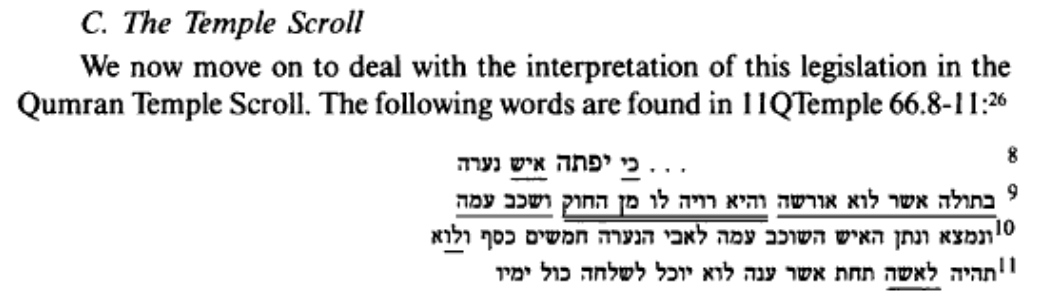
\includegraphics[width=12cm]{temple_scroll1}

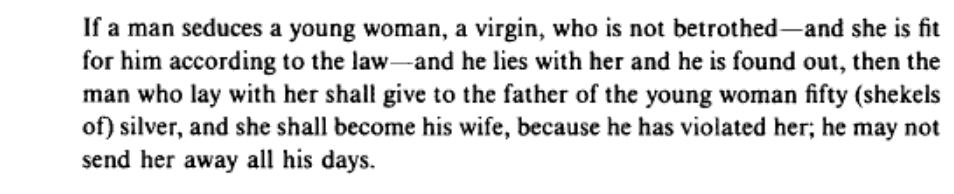
\includegraphics[width=12cm]{dead_sea_scrolls}

Here professor Hiebert states:
\begin{quote}
What is the significance of the scroll writer's harmonization of these two laws? The answer to that question appears to be that he regards the passages in Deuteronomy and Exodus as two case descriptions dealing with similar situations--possibly, as Yigael Yadin suggests, because to the writer there is a degree of imposition involved, whether an unbetrothed virgin is seduced or is raped. I seems that he would in neither case consider her to be a wholly willing party to the offense. Evidence for that assumption may be adduced from the fact that any suggestion of culpability on the part of the young woman described in the passage in 11QTemple is, as has already been mentioned, avoided through the use of the singular\begin{hebrew}ונמצא\end{hebrew}. This interpretation by the writer of the scroll could be colored by several pieces of biblical legis-lation dealing with sexual offenses involving virgins. His line of reasoning might be this: according to Deut 22:23-24, a betrothed virgin who is seduced must die, whereas according to vv 25-27 a betrothed virgin who is raped shall live; turning with this distinction in mind to cases involving an unbetrothed virgin, the fact that an unbetrothed virgin who is seduced (Exod 22:15-16) is not sentenced to death any more than one who is raped (Deut 22:28-29) must mean the former, like the latter, is to be reckoned as having been forced--presumably because an betrothed virgin would not yet, in all probability have reached the age of accountable adulthood.
\end{quote}


Rather than suppose that there is a degree of imposition in the seduction in exodus we would propose another solution: namely that there is no imposition in Deuteronomy 22:28-29 because it isn't about rape. 
Rather than the singular verb implying a lack of culpability for the young woman because she was forced, the singular verb implies a lack of culpability from a legal standpoint because she is not punished and is indeed--as professor Hiebert observes--probably quite young and therefore possible excused from culpability due to here lack of maturity. However, if the seduction was done before the age of sexual maturity the damages would have to be accounted for and this is not directly addressed in the Torah--however a seduction in that case is unlikely--so we would assume the Biblical writer addresses the general straightforward case, just as David gave a different ruling than the law for the malicious theft of the lamb by the rich man here we assume it to be speaking of a general case to give an example or paradigm for interpreting the more specific cases. 
In addition we want to observe that the writer of the temple scroll has deleted the only word that might imply this is rape "taphas" \begin{hebrew}יתפשה\end{hebrew}. If he wanted to imply this was rape he would have used that word (if "taphas" can even mean "rape") or a stronger one to clarify. 



\subsection{Philo Judaeus Combines The Laws}

\begin{quote}
Philo Judaeus's treatment of the biblical legislation under consideration comes in Spec. 3.11 65-71, where Deut 22:28-29 and Exod 22:15-16 are combined, as they are in 11QTemple, to produce a single case study. In this passage the offense is ssociated with terms which connote violence. (\begin{greek}ἁρπάζω, βιάζομαι\end{greek}) and with those which are rather indefinite in that regard but which are often used when seduction is implied ( [fix]).
\end{quote}
XI. (64) But if any one should offer violence to a widow after her husband is dead, or after she has been otherwise divorced from him, and defile her, committing a lighter offence than adultery, and one that may perhaps be about half as serious, he shall not indeed be liable to the punishment of death, but he shall be impeached for violence, and insolence, and intemperance, having thus adopted the most infamous conduct as if it had been the most creditable; and the tribunal of the judge shall decide and condemn him to the penalty that he deserves to suffer. (65) Again, seduction is an offence which is similar and nearly related to adultery, as they are both sprung from one common mother, incontinence. But some of those persons who are accustomed to dignify shameful actions by specious names, call this love, blushing to confess the real truth concerning its character. But, nevertheless, though it may be akin to it, it is not in every respect similar to it, because it is an offence that does not spread so as to affect many families, as is the case with adultery, but it is limited to one house alone, that of the virgin who has been seduced. (66) Therefore we must say to a man who desires to enjoy a virgin who is a free-born citizen, "My good man, rejecting your shameless rashness and audacity, the sources of treachery and faithlessness, and all such feelings, do not allow yourself to be discovered to be wicked, either openly or secretly, (67) but if, indeed, you have any legitimate feeling of love for the maiden in your soul, go to her parents, if they are alive, and if they are not, then go to her brother or to her guardians, or to any other persons who chance to be her protectors, and having discovered to them your feelings towards her, as a free-born man should do, ask her in marriage, and implore them not to account you unworthy. (68) "For no one of those who have the guardianship of the maiden entrusted them could be so base as to oppose an earnest and persevering entreaty, and especially as to refuse you since you, would be found, by strict examination, not to have falsely pretended a passion which you do not feel, or to have conceived only a superficial love for her, but one which is genuine and thoroughly Established."\{4\}\{\#de 22:13.\} (69) But if any one, being insane and frantic, repudiating and discarding all the suggestions of reason, were to submit himself wholly to passion and desire as his masters, and looking, as people say, on might as stronger than right, were to ravish and seduce women, treating free-born women as slaves, and doing acts of war in time of peace, let such a man be led before the judges. (70) And if the damsel who has been forced has a father, let him take counsel and deal with the ravisher about espousing her; then if he refuse to do so, he shall give the damsel a dowry for another husband, being fined in a sum of money sufficient for this purpose. But if he consents and registers her as his wife, let him marry her at once without any delay, confessing a second time that he owes her the same dowry, and let him have no permission to delay or evade the fulfilment of this marriage; both because of his own conduct, in order that the mishap which took place respecting her first connection with a man may be comforted by a firm marriage, which nothing shall ever separate but death. (71) But if the damsel be an orphan and have no father, then let her be asked by the judges whether she is willing to take this man for her husband or not; and whether she agrees to do so or whether she refuses, still let her have the same dowry that the man would have agreed to give her while her father was yet alive.

\url{http://www.earlyjewishwritings.com/text/philo/book29.html}


\begin{greek} ἁρπάζω+ V 4-4-17-11-5=41
Gn 37,33; Lv 5,23; 19,13; Dt 28,31; Jgs 21,21
to snatch away [τι ἔκ τινος] 2 Sm 23,21; to carry off [τινα] Gn 37,33; to seize [τινα] Jgs 21,21; to
captivate, to ravish [τι] Jdt 16,9
→ NIDNTT; TWNT
(→ἀν-, δι-, ἐξ-, συν-) 
\end{greek}

Corresponding Hebrew Words
harpazo H1497 gazal
harpazo H2862 chataph
harpazo H2963 taraph qal.,pu.
harpazo H3920 lakhad

\begin{greek}
βιάζομαι+ V 4-6-0-1-6=17
Gn 33,11; Ex 19,24; Dt 22,25.28; JgsA 13,15
to urge, to insist, to constrain [τινα] Gn 33,11; to force [τινα] Ex 19,24; to lay hands upon, violate [τινα]
Est 7,8; to break violently into [τι] 2 Mc 14,41; to constrain to [+inf.] Ex 19,24
Cf. HELBING 1928, 13; SPICQ 1978a, 189-194; →TWNT
(→ἀπο-, δια-, ἐκ-, κατα-, παρα-) 
\end{greek}
Corresponding Hebrew Words
biazo H2040 haras
biazo H2388 chazaq hi.
biazo H3533 kavash
biazo H6113 atsar
biazo H6484 patsar
biazo H6555 parats
biazo H8610 taphas


 Only one of the words Josephus uses could be interpreted as rape and do not mean that in the LXX. Both of the stronger words philo uses could mean rape but also have other meanings in the LXX and the word “Biazo” he uses seems to have the woman as the direct object which has a pattern of making it “urging” rather than force: https://studybible.info/search-interlinear/strongs/G971 The word translated “ravish” could mean also mean “to snatch away or to carry off” implying try to take her sexually without compensating her father which leads me to my next point:


Josephus, Dead sea scrolls and Philo consider this to be seduction (at least partially) and put the two laws together. 

Either we are left with the idea that this primitive culture didn’t have a concept of what rape was and considered it was the same as seduction or we have to distinguish the two. Deut 22:26 suggests they did have this concept and it was strong enough to compare to murder. Also if we don’t distinguish rape and seduction we are left with the idea of that the woman is culpable in this situation. Since the rapist is not punished for his use of force we either must conclude that the woman got what she deserved by leaving home unprotected or we have to say that the Bible does not punish rape. Since Josphus, Philo and maybe even the people who wrote the dead sea scrolls had the septuagint they would have known that the same word “Biazo” is used in Deut 22:28 and Deut 22:25 and this would mean that they must have seen those words differently because they are used differently. You can reasonably combine the two laws together with my view: that this lacked the consent of the father but was not rape, hence it is identical with seduction in Exodus 22:15-16 and can be combined, otherwise, again we are left with a problem of a Bible that doesn’t care about rape when the culture obviously did--even more so than ours.



If any one has been espoused to a woman as to a virgin, and does not afterward find her so to be, let him bring his action, and accuse her, and let him make use of such indications 1 to prove his accusation as he is furnished withal; and let the father or the brother of the damsel, or some one that is after them nearest of kin to her, defend her If the damsel obtain a sentence in her favor, that she had not been guilty, let her live with her husband that accused her; and let him not have any further power at all to put her away, unless she give him very great occasions of suspicion, and such as can be no way contradicted. But for him that brings an accusation and calumny against his wife in an impudent and rash manner, let him be punished by receiving forty stripes save one, and let him pay fifty shekels to her father: but if the damsel be convicted, as having been corrupted, and is one of the common people, let her be stoned, because she did not preserve her virginity till she were lawfully married; but if she were the daughter of a priest, let her be burnt alive. If any one has two wives, and if he greatly respect and be kind to one of them, either out of his affection to her, or for her beauty, or for some other reason, while the other is of less esteem with him; and if the son of her that is beloved be the younger by birth than another born of the other wife, but endeavors to obtain the right of primogeniture from his father's kindness to his mother, and would thereby obtain a double portion of his father's substance, for that double portion is what I have allotted him in the laws, - let not this be permitted; for it is unjust that he who is the elder by birth should be deprived of what is due to him, on the father's disposition of his estate, because his mother was not equally regarded by him. He that hath corrupted a damsel espoused to another man, in case he had her consent, let both him and her be put to death, for they are both equally guilty; the man, because he persuaded the woman willingly to submit to a most impure action, and to prefer it to lawful wedlock; the woman, because she was persuaded to yield herself to be corrupted, either for pleasure or for gain. However, if a man light on a woman when she is alone, and forces her, where nobody was present to come to her assistance, let him only be put to death. Let him that hath corrupted a virgin not yet espoused marry her; but if the father of the damsel be not willing that she should be his wife, let him pay fifty shekels as the price of her prostitution.

josephus:

\url{http://www.perseus.tufts.edu/hopper/text?doc=Perseus\%3Atext\%3A1999.01.0145\%3Abook\%3D4\%3Awhiston+chapter\%3D8\%3Awhiston+section\%3D23}

josephus in greek:

\url{http://www.perseus.tufts.edu/hopper/text?doc=Perseus\%3Atext\%3A1999.01.0146\%3Abook\%3D4\%3Awhiston+chapter\%3D8\%3Awhiston+section\%3D23}

The two words in red he uses in LSJ:

\url{http://www.perseus.tufts.edu/hopper/morph?l=u\%28\%2Fbrews&la=greek&can=u\%28\%2Fbrews0&prior=th=s#lexicon}

\url{http://www.perseus.tufts.edu/hopper/morph?l=fqei\%2Fras&la=greek&can=fqei\%2Fras1&prior=o(#lexicon}


Only one of those two words (in red) can mean rape and it doesn't seem to mean that in the septuagint lexicon:


The word he uses in the septuagint context and lexicons: \url{https://studybible.info/search-interlinear/strongs/5196}


\begin{greek} ὕβρις,-εως+ \end{greek} N3F 1-0-32-16-13=62 Lv 26,19; Is 9,8; 10,33; 13,11(bis) insolence, pride, arrogance Est 4,17d; shame, insult, mistreatment Sir 10,8; hardship 3 Mc 3,25 \begin{greek} ἡ ὕβρις τῆς ἰσχύος αὐτῆς hybris, \end{greek} i.e. haughty behaviour, (on account) of her strength Ez 33,28 *Mi 6,10 \begin{greek} ὕβρεως \end{greek} (of) pride-\begin{hebrew}זדון\end{hebrew}  for MT\begin{hebrew} רזון \end{hebrew}emaciation; *Prv 14,10 \begin{greek} ὕβρει \end{greek} (with) pride-\begin{hebrew}זד\end{hebrew} for MT\begin{hebrew}זר\end{hebrew}stranger Cf. BERTRAM 1964, 29-38; →NIDNTT; TWNT 

http://www.glasovipisma.pbf.rs/phocadownload/knjige/greek%20lexicon%20for%20the%20septuagint.pdf


%place where I copied the temple scroll stuff from

G Dinah 
  εκοιμήθη in Genesis 30:16 (going to bed in story of the mandrakes) is the same as in Gen 34:2 


Luke 20:29 V-APA-NMS
\begin{greek}
GRK: ὁ πρῶτος λαβὼν γυναῖκα ἀπέθανεν
\end{greek}
NAS: and the first took a wife


Deuteronomy 22:22 root word for “humbled” is the same in Gen 34:2

 https://studybible.info/interlinear/Deuteronomy%2022:22



 Deu 22:24 word for “humbled” is the same in Gen 34:2 (in the Piel form)


Gen 30:15 word for “sleep with” is the same in Gen 34:2 (in the Qal form)

Then ye shall bring them both out unto the gate of that city, and ye shall stone them with stones that they die; the damsel, because she cried not, being in the city; and the man, because he hath humbled H6031 his neighbour's wife: so thou shalt put away evil from among you.




\section{Word Difference: Distinction Between Violence and Lack of Mutuality}
\begin{quote}
This is distinct from ḥāzaq, which describes a forcible overpowering. Daniel Block notes that, unlike the law in verses 25-27, this law has neither a cry for help, nor an account of male violence.[7] It’s likely that the woman in verses 28-29 experienced overwhelming persuasion, perhaps an erosion of her resolve, but not necessarily a sexual assault.
\url{https://cbmw.org/topics/sex/did-old-testament-law-force-a-woman-to-marry-her-rapist/#_ftnref8}
\end{quote}
The word "taphas" (in Qal perfect form) then "shakab" in Deut 22:28 is different than what is used in Deut 22:23 which only has "shakab." Since I think different words used in situations near to each other say something about the situation and 22 is mutual I think this is not mutual to a certain extent. However, since it is also different than the word used to describe force and rape in Deut 28:25 I think it is not violent. This will be explained. 

Here we see some examples of taphas being used in a non-violent from Gesenius. In this definition Jer 40:10 uses taphas in the Qal perfect form which is the same form that it appears in Deuteronomy 22:28:
\begin{quote}
“to hold as a city, hence to handle, to wield as a sickle, a bow, an oar, the harp . . .” 
\end{quote}
This is Gesenius \#2 definition for "taphas" and does not imply holding by violence. Also to “handle the law” is under the same definition. Gesenius’s second definition seems to imply this could be a non-mutual act yet it also implies it isn't violent (playing the harp and handling the law). While holding a city could be a violent act, here it seems to be just the occupying and living in the city that is referred to:
\begin{quote}
10 As for me, I am staying at Mizpah to represent you before the Chaldeans who come to us; but as for you, gather wine and summer fruits and oil, and store them in your vessels, and live in the towns that you have taken over.” (Jeremiah 40:10 NRSV)
\end{quote}

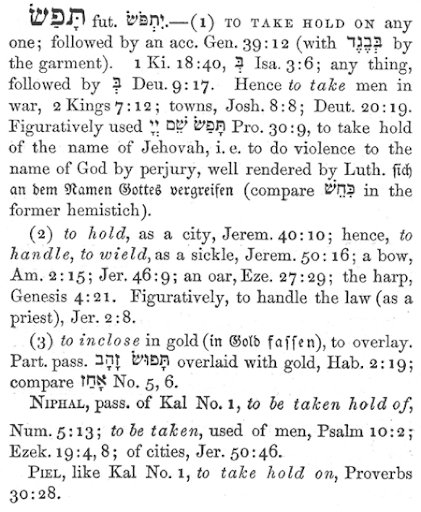
\includegraphics[width=10cm]{taphas}
\newline
Strong’s says it could be used to describe manipulation or "unwarrantable use" not even non-mutuality:

 \begin{hebrew} תּפשׂ  \end{hebrew}
\begin{quote}
taphas \newline
taw-fas' \newline
A primitive root; to manipulate, that is, seize; chiefly to capture, wield; specifically to overlay; figuratively to use unwarrantably
\newline
[KJV Usage:] catch, handle, (lay, take) hold (on, over), stop, X surely, surprise, take. \newline
\url{https://www.blueletterbible.org/lang/lexicon/lexicon.cfm?Strongs=H8610&t=KJV}
\end{quote}

As does Brown-Driver-Briggs' Hebrew Definitions (wield, use skillfully) There are some disagreements with this. For instance, Mary Anna Bader writes this response to Lyn Bechtel:

\begin{quote}
I do not find "taphas" to be used in contexts describing mutual consensual relations anywhere in the Hebrew Bible. Let us consider those passages. When the verb "taphas" is used in Genesis 39:12, Potiphar's wife seized or caught hold of Joseph by his garment as she begged him to lie with her. Anything but mutuality is described here. Bechtel's Point that this verb is indicative of mutuality can be substantially undermined. Potiphar's wife, we would say today, was sexually harassing Joseph. He was not willing to participate in a sexual liaison with the wife of his master. 2 Kins 7:12 uses the verb "taphas" when Elisha described the ploy the Arameans had prepared, capturing the Israelites alive and then infiltrating the city. 
\url{https://www.answering-christianity.com/karim/Karim_-_articles_islamic_answers_-_part_3/Biblical\%20Laws\%20on\%20Rape\%20-\%20commentary\%20Deuter\%2022_\%2028-29.doc}
\end{quote}

Contrary to Mary Anna Bader there is at least one clear exception to this non-mutuality in Eze 29:7. Here it is used to describe a grasping onto for help which is not an action that was intended to be non-mutual since Israel had an alliance with Egypt:
\begin{quote}
6 Then all the inhabitants of Egypt shall know
    that I am the Lord
because you were a staff of reed
    to the house of Israel;
7 when they \textbf{grasped} you with the hand, you broke,
    and tore all their shoulders;
and when they leaned on you, you broke,
    and made all their legs unsteady.
    (Ezekiel 29:6-7 NRSV)
\end{quote}
Neither is it saying Egypt "broke" Israel in response but it was Egypt's unwillingness to come to their aid that warrants their description as a "staff of reed" which breaks under the house of Israel's grasp. Maybe it is using this just in terms of the analogy of grabbing a reed (which would be a non-mutual act since the reed does not have a will of its own) However, Egypt is described as being at fault for breaking since the next part of the prophecy is about their punishment. This makes us think that mutuality was intended in the grasp.

\section{Two Levels of Consent}
However, is the father's consent required in the law? Yes, in addition to that the woman's consent is required to get married. Here we will go over the reasons why there are two levels of consent required for marriage: 1 woman, 2 woman’s guardian

\subsection{Woman's Consent Was Required}

1. A woman’s consent was required because of the laws against capturing and holding people as slaves. (see also section \ref{bible mention rape}) If you couldn't capture people and you couldn't hold them then you couldn't force them to marry or have sex with you and if slaves were able to run away everyone was able to run away a fortiori. (this is also know as the "rule of heavy and light")
\begin{quote}
 Whoever kidnaps a person, whether that person has been sold or is still held in possession, shall be put to death. (Ex 21:16 NRSV)
\end{quote}
\begin{quote}
21 You shall not wrong or oppress a resident alien, for you were aliens in the land of Egypt. 22 You shall not abuse any widow or orphan. 23 If you do abuse them, when they cry out to me, I will surely heed their cry; 24 my wrath will burn, and I will kill you with the sword, and your wives shall become widows and your children orphans. (Ex 22:21-24 NRSV)
\end{quote}
\begin{quote}
You shall not oppress a resident alien; you know the heart of an alien, for you were aliens in the land of Egypt. (Ex 23:9 NRSV)
\end{quote}
\begin{quote}
15 Slaves who have escaped to you from their owners shall not be given back to them. 16 They shall reside with you, in your midst, in any place they choose in any one of your towns, wherever they please; you shall not oppress them. (Deut 23:15-16 NRSV)
\end{quote}

\subsection{Father's Consent Was Required}

2. Women in their father’s house couldn't consent without their father. Father’s are responsible for their daughter’s sexual and marital behavior:
\begin{quote}
Do not profane H2490 your daughter by making her a prostitute, that the land not become prostituted and full of depravity. (Lev 19:29 NRSV)
\end{quote}

Gesenius describes this as "to lay open, to give access to ["to profane from the idea of opening"], hence--(a) Lev 19:29 to prostitute one's daughter\newline
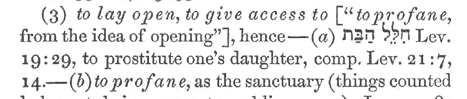
\includegraphics[width=10cm]{chalal}
\url{https://www.blueletterbible.org/lang/lexicon/lexicon.cfm?Strongs=H2490&t=KJV}

The same word (although a slightly different Strong's number) is used in Lev 21:7:
\begin{quote}
They shall not marry a prostitute or a woman who has been defiled; H2491 neither shall they marry a woman divorced from her husband. For they are holy to their God, (Lev 21:7 NRSV)
\end{quote}
Also see here for more explanation of the sexual laws:
\begin{quote}
Do not intermarry with them, giving your daughters to their sons or taking their daughters for your sons,
(Deuteronomy 7:3 NRSV)
\end{quote}

\url{https://kingdomofgodcommunes.org/2019/02/03/gesenius-and-leviticus-1929/}

That’s why they had to make a law specifically for the situation when the guardians were dead:

\begin{quote}
10 When you go out to war against your enemies, and the Lord your God hands them over to you and you take them captive, 11 suppose you see among the captives a beautiful woman whom you desire and want to marry, 12 and so you bring her home to your house: she shall shave her head, pare her nails, 13 discard her captive’s garb, and shall remain in your house a full month, mourning for her father and mother; after that you may go in to her and be her husband, and she shall be your wife. 14 But if you are not satisfied with her, you shall let her go free and not sell her for money. You must not treat her as a slave, since you have dishonored her. (Deut 21:10-14 NRSV)
\end{quote}

There is even a law stating that the father could annul the vow of a woman still in household, interestingly enough the guilt of the vows may be transferable from the woman to the father (just like they were transferable from the woman to the husband in verse 15) This may suggest a sort of unity that existed under law where the father or husband could take responsibility for the woman in certain cases. 
\begin{quote}
1 Then Moses said to the heads of the tribes of the Israelites: This is what the Lord has commanded. 2 When a man makes a vow to the Lord, or swears an oath to bind himself by a pledge, he shall not break his word; he shall do according to all that proceeds out of his mouth.

3 When a woman makes a vow to the Lord, or binds herself by a pledge, while within her father’s house, in her youth, 4 and her father hears of her vow or her pledge by which she has bound herself, and says nothing to her; then all her vows shall stand, and any pledge by which she has bound herself shall stand. 5 But if her father expresses disapproval to her at the time that he hears of it, no vow of hers, and no pledge by which she has bound herself, shall stand; and the Lord will forgive her, because her father had expressed to her his disapproval.

6 If she marries, while obligated by her vows or any thoughtless utterance of her lips by which she has bound herself, 7 and her husband hears of it and says nothing to her at the time that he hears, then her vows shall stand, and her pledges by which she has bound herself shall stand. 8 But if, at the time that her husband hears of it, he expresses disapproval to her, then he shall nullify the vow by which she was obligated, or the thoughtless utterance of her lips, by which she bound herself; and the Lord will forgive her. 9 (But every vow of a widow or of a divorced woman, by which she has bound herself, shall be binding upon her.) 10 And if she made a vow in her husband’s house, or bound herself by a pledge with an oath, 11 and her husband heard it and said nothing to her, and did not express disapproval to her, then all her vows shall stand, and any pledge by which she bound herself shall stand. 12 But if her husband nullifies them at the time that he hears them, then whatever proceeds out of her lips concerning her vows, or concerning her pledge of herself, shall not stand. Her husband has nullified them, and the Lord will forgive her. 13 Any vow or any binding oath to deny herself, her husband may allow to stand, or her husband may nullify. 14 But if her husband says nothing to her from day to day, then he validates all her vows, or all her pledges, by which she is obligated; he has validated them, because he said nothing to her at the time that he heard of them. 15 But if he nullifies them some time after he has heard of them, then he shall bear her guilt.(Numbers 30:1-15 NRSV)
\end{quote}

The state that the woman was in--in relation to her guardian--changes the severity of the crime committed (compare to Deut 22:22-24):
\begin{quote}
20 If a man has sexual relations with a woman who is a slave, designated for another man but not ransomed or given her freedom, an inquiry shall be held. They shall not be put to death, since she has not been freed; 21 but he shall bring a guilt offering for himself to the Lord, at the entrance of the tent of meeting, a ram as guilt offering. 22 And the priest shall make atonement for him with the ram of guilt offering before the Lord for his sin that he committed; and the sin he committed shall be forgiven him. (Lev 19:20-22 NRSV)
\end{quote}

Philo compares seduction to rape seeming to imply it is not consensual because the father was not consulted. He even says of it "acts of war done in times of peace." It is interesting to note that "taphas" is sometimes used to describe the capture of people in war but we have not found it to mean a violent seizure usually it seems to be stated that the victims went without fighting with soldiers since they realized they were outnumbered. Along with Deuteronomy 21:10-14 which describes what to do when a woman's guardians are dead it's context is a state of war. Hence, not consulting the guardians is like performing marriage in a time of war, hence like Philo says: acts of war in times of peace.
\begin{quote}
XI. (64) But if any one should offer violence to a widow after her husband is dead, or after she has been otherwise divorced from him, and defile her, committing a lighter offence than adultery, and one that may perhaps be about half as serious, he shall not indeed be liable to the punishment of death, but he shall be impeached for violence, and insolence, and intemperance, having thus adopted the most infamous conduct as if it had been the most creditable; and the tribunal of the judge shall decide and condemn him to the penalty that he deserves to suffer. (65) Again, seduction is an offence which is similar and nearly related to adultery, as they are both sprung from one common mother, incontinence. But some of those persons who are accustomed to dignify shameful actions by specious names, call this love, blushing to confess the real truth concerning its character. But, nevertheless, though it may be akin to it, it is not in every respect similar to it, because it is an offence that does not spread so as to affect many families, as is the case with adultery, but it is limited to one house alone, that of the virgin who has been seduced. (66) Therefore we must say to a man who desires to enjoy a virgin who is a free-born citizen, "My good man, rejecting your shameless rashness and audacity, the sources of treachery and faithlessness, and all such feelings, do not allow yourself to be discovered to be wicked, either openly or secretly, (67) but if, indeed, you have any legitimate feeling of love for the maiden in your soul, go to her parents, if they are alive, and if they are not, then go to her brother or to her guardians, or to any other persons who chance to be her protectors, and having discovered to them your feelings towards her, as a free-born man should do, ask her in marriage, and implore them not to account you unworthy. (68) "For no one of those who have the guardianship of the maiden entrusted them could be so base as to oppose an earnest and persevering entreaty, and especially as to refuse you since you, would be found, by strict examination, not to have falsely pretended a passion which you do not feel, or to have conceived only a superficial love for her, but one which is genuine and thoroughly Established."\{4\}\{\#de 22:13.\} (69) But if any one, being insane and frantic, repudiating and discarding all the suggestions of reason, were to submit himself wholly to passion and desire as his masters, and looking, as people say, on might as stronger than right, were to ravish and seduce women, treating free-born women as slaves, and doing acts of war in time of peace, let such a man be led before the judges. (70) And if the damsel who has been forced has a father, let him take counsel and deal with the ravisher about espousing her; then if he refuse to do so, he shall give the damsel a dowry for another husband, being fined in a sum of money sufficient for this purpose. But if he consents and registers her as his wife, let him marry her at once without any delay, confessing a second time that he owes her the same dowry, and let him have no permission to delay or evade the fulfilment of this marriage; both because of his own conduct, in order that the mishap which took place respecting her first connection with a man may be comforted by a firm marriage, which nothing shall ever separate but death. (71) But if the damsel be an orphan and have no father, then let her be asked by the judges whether she is willing to take this man for her husband or not; and whether she agrees to do so or whether she refuses, still let her have the same dowry that the man would have agreed to give her while her father was yet alive.
(Philo)
\end{quote}

\section{Under Another's Authority}

This word is used in Deut 22:23,25,28 to imply these women were under someone’s authority. \url{https://studybible.info/search-interlinear/strongs/3816/start/90} however this word is not used in Deuteronomy 22:22 implying the situation there is something the woman is expected to be fully responsible for unlike in 28. A damsel is said to be betrothed in these verses in the Hebrew:
23, 25, 27, and 28

In the septuagint it doesn't translated the 
The word betrothed is 

Another possibility is that they are using this 

\begin{quote}
1 Then Moses said to the heads of the tribes of the Israelites: This is what the Lord has commanded. 2 When a man makes a vow to the Lord, or swears an oath to bind himself by a pledge, he shall not break his word; he shall do according to all that proceeds out of his mouth.
3 When a woman makes a vow to the Lord, or binds herself by a pledge, while within her father’s house, in her youth, 4 and her father hears of her vow or her pledge by which she has bound herself, and says nothing to her; then all her vows shall stand, and any pledge by which she has bound herself shall stand. 5 But if her father expresses disapproval to her at the time that he hears of it, no vow of hers, and no pledge by which she has bound herself, shall stand; and the Lord will forgive her, because her father had expressed to her his disapproval. (Numbers 30:1-5 NRSV)
\end{quote}

\begin{quote}
 7 and her husband hears of it and says nothing to her at the time that he hears, then her vows shall stand, and her pledges by which she has bound herself shall stand. 8 But if, at the time that her husband hears of it, he expresses disapproval to her, then he shall nullify the vow by which she was obligated, or the thoughtless utterance of her lips, by which she bound herself; and the Lord will forgive her. 9 (But every vow of a widow or of a divorced woman, by which she has bound herself, shall be binding upon her.) 10 And if she made a vow in her husband’s house, or bound herself by a pledge with an oath, 11 and her husband heard it and said nothing to her, and did not express disapproval to her, then all her vows shall stand, and any pledge by which she bound herself shall stand. 12 But if her husband nullifies them at the time that he hears them, then whatever proceeds out of her lips concerning her vows, or concerning her pledge of herself, shall not stand. Her husband has nullified them, and the Lord will forgive her. 13 Any vow or any binding oath to deny herself, her husband may allow to stand, or her husband may nullify. 14 But if her husband says nothing to her from day to day, then he validates all her vows, or all her pledges, by which she is obligated; he has validated them, because he said nothing to her at the time that he heard of them. 15 But if he nullifies them some time after he has heard of them, then he shall bear her guilt.
 (Number 30:7-9 NRSV)
\end{quote}

\begin{quote}
\begin{greek} παῖς, παιδός+ N3M/F 126-184-39-47-74=470
Gn 9,25.26.27; 12,16; 14,15
child (in relation to parents) Prv 29,15; slave, servant Gn 9,25; courtier, attendant 1 Sm 22,17; servant
(of humans in relation to God) Is 41,8; girl, young lady Gn 24,28; girl, slave, maid Ru 2,6; παῖδες
children Prv 4,1
ἐκ παιδός from childhood, from youth Gn 46,34
*Gn 26,18 οἱ παῖδες the servants-עבדי) Sam. Pent.) for MT בימי in the days of; *Gn 47,21 εἰς παῖδας for \end{greek}
servants\begin{hebrew} -עבדים/ל for MT ערים/ל into \end{hebrew} the cities; *Jos 7,7 \begin{greek} διεβίβασεν ὁ παῖς σου \end{greek} your servant brought over
\begin{hebrew}
 עבדך
העביר for MT העביר העברת you surely brought over; 
 \end{hebrew}
\begin{greek}  *Jer 47(40),9 τῶν παίδων of the servants of \end{greek}
\begin{hebrew}
  מעבדי
for MT עבוד/מ 
\end{hebrew}
\begin{greek}
from serving, see also 2 Kgs 25,24; *Prv 1,4 παιδὶ δὲ νέῳ but to a young child, but to
a little child double transl. of MT
\end{greek}
\begin{hebrew}
 נער young man
\end{hebrew}
Cf. AMUSIN 1986 132-136.145-146; DANIEL, S. 1966 103.104; HARL 1986a, 68.143.200; HEINEN 1984,
1287-1295; KATZ 1956, 268-269; LARCHER 1983, 245-246; LE BOULLUEC 1989, 109; SCHOLL 1983 7-
8.15; SPICQ 1978b, 220-224; STANTON 1988, 475-476; WEVERS 1990 46; 1993 319.567; 1995 173.357;
→NIDNTT; TWNT 

\url{http://www.glasovipisma.pbf.rs/phocadownload/knjige/greek\%20lexicon\%20for\%20the\%20septuagint.pdf}
\end{quote}


Virgin word usage https://studybible.info/search-interlinear/strongs/3933

 Deuteronomy 22:23, 28 are the only ones that have this word in the 22:22-30 section

\begin{greek}
παρθένος,-ου+ \end{greek} N2F 16-10-17-12-12=67
Gn 24,14.16(bis).43.55
virgin Jgs 19,24; virgin (as adj.) Lv 21,3; young woman Ez 9,6; a girl of marriage-able age Gn 24,14
Cf. DODD 1976, 301-305; DOGNIEZ 1992, 257; DUBARLE 1978, 370-371; FORD 1966, 293-299; GESE
1971, 88; HARL 1986a, 200; HORSLEY 1987, 222-226; SEELIGMAN 1948 118-119(Is 7,14); SPICQ 1982,
519-521; WEGNER 1992, 112-113; →NIDNTT; TWNT


\section{This Is Not Force}

If this is non-consensual it is because the daughter cannot fully consent without her father. Here are some more reasons for this:
\subsection{Different situation}
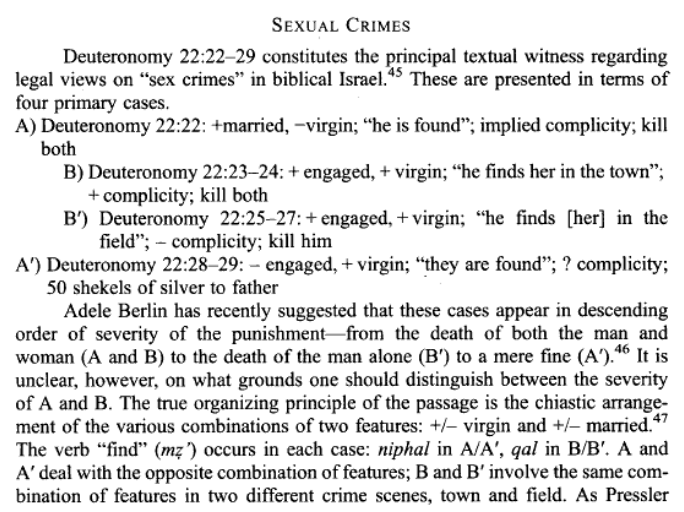
\includegraphics[width=10cm]{sexual_crimes} \newline
Here is a diagram of the situation by Robert S. Kawashima who believes that Deuteronomy 22:28 covered both complicity and non-complicity by the man and the woman (hence both rape and seduction). He claims "The true organizing principle of the passage is the chiastic arrangement of the various combination of two features: +/- virgin and +/- married. . . A and A' deal with the oppsite combination of features; B and B' the same combination of features in two different crime scenes town and field." If we add in complicity as third variable, for married, virigin, complicity, under his schema we get 5 different conditions since the last condition would be assumed to cover both connsent and lack thereof. We can give these numbers in a binary system for - = 0 and + = 1 \newline


\begin{tabular}{ c c c c }
 + & - & + & =5\\ 
 + & + & + & =7 \\  
 + & + & - & =6 \\
 - & + & + & =3 \\
 - & + & - & =2 \\
\end{tabular} \newline


My adaptation would only include given that I think there is complicity in deuteronomy 22:28 between the man and the woman: \newline 
\begin{tabular}{ c c c c }
 + & - & + & =5\\ 
 + & + & + & =7 \\  
 + & + & - & =6 \\
 - & + & + & =3 \\
\end{tabular} \newline 

In addition to the problems we have already found with "- + -" and there being no real punishment for rape, it is interesting that even with this included scenario quite a few scenarios are missing. We can count the total scenarios like a binary number: \newline


\begin{tabular}{ c c c c }
 - & - & - & =0\\ 
 - & - & + & =1 \\  
 - & + & - & =2 \\
 - & + & + & =3 \\
 + & - & - & =4 \\
 + & - & + & =5 \\  
 + & + & - & =6 \\
 + & + & + & =7 \\

\end{tabular} \newline

Since there are 8 scenarios, and Kawashima includes 2, 3, 5, 6, 7 (total 5), 4 scenarios are missing: 0, 1, 4, 7. These missing scenarious include. 
0 - - - an unmarried non-virgin is raped by a man \newline 
1 - - + an unmarried non-virgin is slept with by a man \newline
4 + - - a married non-virgin is raped by a man \newline
7 + + + a married virgin is slept with by a man \newline

The Bible elsewhere does not address unmarried non-virgins, perhaps because it wasn't a common occurrence. Assumably we are supposed to derive the punishment from the observing the punishments for the unmarried virgins. A married non-virgin is who is raped by a man is a useless scenario since we know that the maximum punishment of death would be applied given the same status covered in Deuteronomy 22:22 but with consensual adultery. The scenario of a married virgin is slept with by a man is also useless since we already know the penalty is death given be the same situation with the non-virgin. The question is is his scenario number 2 also also useless? i.e. an unmarried virgin raped by a man. I would argue in the affirmative because of the very libertarian laws governing individuals in the Torah and the absolutely abhorrence of rape in the culture and capture/slavery in the Torah (see previous explanation \ref{bible mention rape}) would imply that rape deserved death. Here, are some reasons why scenario number two is not needed and "taphas" only implies lack of consent from the father not from the woman:

1. Right after Deuteronomy 22:29, verse 30 “you shall not take your father’s wife” so it continues the theme of the rights of fathers after it started in Deuteronomy 22:28 (switching there from the rights of husbands)

2. Deuteronomy 22:28 uses a different word that Deuteronomy 22:25 implying it is not violent.

3. The word “taphas” can mean “take” as in taking a city or taking men in battle this is why it is the rights of fathers which continues in Deut 22:30 because he is “taking” her from her father. 
Given that the context is the same and this set of laws should include Deuteronomy 22:30, we can say with some confidence that complicity between the man and the woman is implied in verse 28, as in 22 and 30. Kiel and Delitzsch note:
\begin{quote}
Deuteronomy 22:30
A man shall not take his father's wife, nor discover his father's skirt.
(or Deuteronomy 23:1) This verse, in which the prohibition of incest is renewed by a repetition of the first provision in the earlier law (Leviticus 18:7-8), is no doubt much better adapted to form the close of the laws of chastity and marriage, than the introduction to the laws which follow concerning the right of citizenship in the congregation of the Lord.
\end{quote}

4. The situation implied complicity like in 22:22. No longer is it stated whether the woman cried out or whether she was in the city or the countryside which would leave the complicity implied like in Deuteronomy 22:22 since the woman now has to marry the person she slept with as does the man.
In addition to this, the context of Deuteronomy 22:22 is the same as Deuteronomy 22:28-30 meaning the default would be to assume that complicity is implied it is only the word "taphas" which may suggest otherwise. 

5. If we are to say this is rape since “taphas” is associated with war then we must say Deut 21:10-14 means rape as well since there is no information given about the woman’s consent. This is quite an undesirable conclusion and would mean that there was literally no penality for raping a woman captured in war. 

6. There is the possibility of mutuality with taphas: “When they took hold H8610 of thee by thy hand, thou didst break, and rend all their shoulder: and when they leaned upon thee, thou brakest, and madest all their loins to be at a stand.” Eze 29:7

7. If taphas has the implication of taking people in war then I would argue that for the israelites this did not imply rape since the Israelites did not do this in war (as is also testified in Deu 21) so therefore consent of the woman is implied. The implication of “war” just refers to not consulting the father like in Deuteronomy 21:10-14 Also Philo connects seduction to acts of war.

8. Complicity is sometimes not stated clearly, it is only implied like in Deuteronomy 22:22, but non complicity is usually clearly stated in this situation.

\subsection{Word Difference}

In Deu 22:24 word for “humbled” is the same (Piel form) which does not mean rape.

Taphas means “to hold” while “chazaq” means “to hold fast.” Taphas does not have the context of force unlike chazaq which means to “bind tightly” or “be strong” or “overpower.” I think the reason why they didn’t use “laqach” is because it could be mistaken for “taking a wife” properly without more context given.  


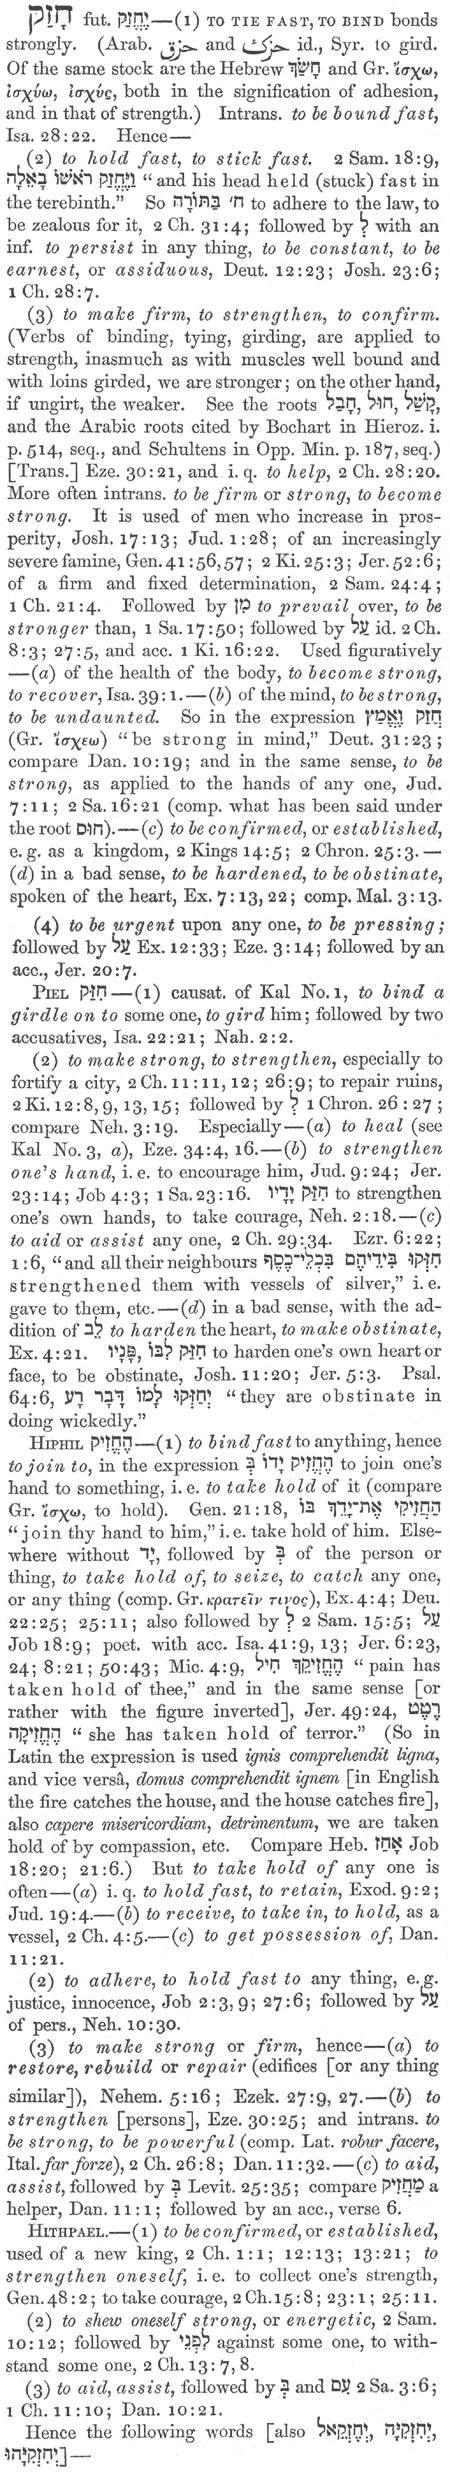
\includegraphics[width=4cm]{chazak}


\subsection{Word Definition Must Rely on Context}


\subsubsection{May be a mistake to rely on words, instead rely on context. Even “chazdaq” can be used non violently or violently in the same word form}


Stem: Hiphil
Aspect: Imperfect

Jdg 19:4
And his father in law, the damsel's father, retained H2388 him; and he abode with him three days: so they did eat and drink, and lodged there.



Stem: Hiphil
Aspect: Imperfect

2Ki 4:8
And it fell on a day, that Elisha passed to Shunem, where was a great woman; and she constrained H2388 him to eat bread. And so it was, that as oft as he passed by, he turned in thither to eat bread.



Stem: Hiphil
Aspect: Perfect

Deu 22:25
But if a man find a betrothed damsel in the field, and the man force H2388 her, and lie with her: then the man only that lay with her shall die:


Stem: Hiphil
Aspect: Imperfect
2Sa 13:11
And when she had brought them unto him to eat, he took hold H2388 of her, and said unto her, Come lie with me, my sister.

Stem: Qal
Aspect: Imperfect
2Sa 13:14
Howbeit he would not hearken unto her voice: but, being stronger H2388 than she, forced her, and lay with her.




Taphas (qal imperfect) to hold onto his brother while pleading with him:
Isa 3:6
When a man shall take hold h8610 of his brother of the house of his father, saying, Thou hast clothing, be thou our ruler, and let this ruin be under thy hand:
7 In that day he will protest, saying,
“I cannot cure your ills,
For in my house is neither food nor clothing;
Do not make me a ruler of the people.”


The crime is not connected to force but to humbling as in Deut 21:15 where she has no guardian:

Deu 22:22
If a man be found lying H7901 with a woman married to an husband, then they shall both of them die, both the man that lay H7901 with the woman, and the woman: so shalt thou put away evil from Israel.

Deu 22:29
Then the man that lay H7901 with her shall give unto the damsel's father fifty shekels of silver, and she shall be his wife; because he hath humbled her, he may not put her away all his days.



Gen 34:2
And when Shechem the son of Hamor the Hivite, prince of the country, saw her, he took her, and lay with her, and defiled her. H6031


Deu 21:14
And it shall be, if thou have no delight in her, then thou shalt let her go whither she will; but thou shalt not sell her at all for money, thou shalt not make merchandise of her, because thou hast humbled H6031 her.


Deu 22:24
Then ye shall bring them both out unto the gate of that city, and ye shall stone them with stones that they die; the damsel, because she cried not, being in the city; and the man, because he hath humbled H6031 his neighbour's wife: [but she was betrothed not married] so thou shalt put away evil from among you.


Deu 22:29
Then the man that lay with her shall give unto the damsel's father fifty shekels of silver, and she shall be his wife; because he hath humbled H6031 her, he may not put her away all his days.


Lam 5:11
They ravished H6031 the women in Zion, and the maids in the cities of Judah.


Eze 22:10
In thee have they discovered their fathers' nakedness: in thee have they humbled H6031 her that was set apart for pollution.


Eze 22:11
And one hath committed abomination with his neighbour's wife; and another hath lewdly defiled his daughter in law; and another in thee hath humbled H6031 his sister, his father's daughter.





Oddly enough the word for “force” that can mean rape is used for him forcing his concubine and for his father forcing him to stay there:

Jdg 19:4
And his father in law, the damsel's father, retained H2388 him; and he abode with him three days: so they did eat and drink, and lodged there.


Jdg 19:25
But the men would not hearken to him: so the man took H2388 his concubine, and brought her forth unto them; and they knew her, and abused her all the night until the morning: and when the day began to spring, they let her go.




Also of the concubine:

Jdg 19:25
But the men would not hearken to him: so the man took his concubine, and brought her forth unto them; and they knew her, and abused H5953 her all the night until the morning: and when the day began to spring, they let her go.





Judges uses completely different words when they took themselves wives by force:



Jdg 21:21
And see, and, behold, if the daughters of Shiloh come out to dance in dances, then come ye out of the vineyards, and catch H2414 you every man his wife of the daughters of Shiloh, and go to the land of Benjamin.


Jdg 21:23
And the children of Benjamin did so, and took h5375 them wives, according to their number, of them that danced, whom they caught: h1497 and they went and returned unto their inheritance, and repaired the cities, and dwelt in them.


Same with Samuel:


2Sa 13:11

And when she had brought them unto him to eat, he took hold H2388 of her, and said unto her, Come lie with me, my sister.

2Sa 13:14

Howbeit he would not hearken unto her voice: but, being stronger H2388 than she, forced her, and lay with her.


\subsubsection{The words used for “taking” a wife and “finding” a woman can be used in violent contexts however like “taphas” context is key to decide whether they are violent:}

Laqach can be associated with violence but it is not always used that way, the Qal perfect form:

 Deu 22:14

And give occasions of speech against her, and bring up an evil name upon her, and say, I took H3947 this woman, and when I came to her, I found her not a maid:


 Deu 22:18

And the elders of that city shall take H3947 that man and chastise him;


 Jos 7:24

And Joshua, and all Israel with him, took H3947Achan the son of Zerah, and the silver, and the garment, and the wedge of gold, and his sons, and his daughters, and his oxen, and his asses, and his sheep, and his tent, and all that he had: and they brought them unto the valley of Achor.


 Jos 11:19

There was not a city that made peace with the children of Israel, save the Hivites the inhabitants of Gibeon: all other they took H3947 in battle.



The word for “found” H4672 can even be used in associating with a violent act:

Deu 31:17
Then my anger shall be kindled against them in that day, and I will forsake them, and I will hide my face from them, and they shall be devoured, and many evils and troubles shall befall H4672 them; so that they will say in that day, Are not these evils come H4672 upon us, because our God is not among us?



\section{Things left to decide:}

Richard Abbot writes in his  footnote on Deut. 22:28 the next about the Hebrew word "taphas": 

tâphas, here used in the Qal perfect form with suffix, has a violent or forceful air, hence seize. 2


\section{appendix, Philo, Josephus}

Greek words translated from the qal perfect “taphas” to find what is common between all:
4815

Deu 21:19, Jos 8:23, 2 Kings 14:7, 2 Kings 14:13
\begin{greek}
συλλαμβάνω+ V 23-28-25-15-27=118
Gn 4,1.17.25; 16,4; 19,36
A: to lay hold of, to arrest [τινα] (of pers.) 1 Kgs 13,4; to take, to catch [τινα] (of anim.) Jgs 15,4; to
take, to capture [τι] 2 Kgs 14,7; to conceive [abs.] Gn 4,1; id. [τινα] Ct 3,4; id. [τι] (metaph.) Ps 7,15
P: to be taken (from earth) Jb 22,16
συλλήμψεται μεθ᾽ ἑαυτοῦ he shall take with himself Ex 12,4
*Ct 8,2 τῆς συλλαβούσης με of her who conceived me-◊ילד for MT ◊למד she teaches me?, cpr. Ct 3,4
 (הורתי)
Cf. HELBING 1928, 310; MARGOLIS, M. 1906a=1972 78-79; →NIDNTT; TWNT
\end{greek}


2638

2 Chronicles 25:23
\begin{greek}
καταλαμβάνω+ V 13-31-19-20-43=126
Gn 19,19; 31,23.25; 44,4; Ex 15,9
A: to take, lay hold of [τι] Jgs 7,24; to take, to overtake [τινα] (of God) Jb 5,13; to overtake, to befall
[τινα] (of evil) Gn 19,19; to overtake [τινα] (often after a pursuit) Gn 31,23; to reach [τινα] (of men
reaching God) Mi 6,6; to overtake, to take hold of [τινα] (of sin; metaph.) Ps 39(40),13; to lay hold of, to
come over, to overtake [τινα] (of feelings; metaph.) Ps 68(69),25; to take prisoner [τινα] 2 Chr 25,23; to
take, to capture [τι] (of city) 2 Sm 12,26
to comprehend, to understand [τι] Jb 34,24, cpr. DnLXX 1,20
to find sb doing [τινα +pred.] 1 Ezr 6,8; to detect, to catch in the act of doing (esp. of the detection of
adultery) [τινα] SusLXX 58, see also Jer 3,8 (double transl. of the Hebr.)
M: to seize, to lay hold on [τι] Prv 1,13; to overtake, to take hold of [τινα] (of sin) Jdt 11,11; to take, to
capture [τι] (of city) Nm 21,32; to occupy, to keep [τι] 1 Mc 11,46
P: to be taken, to be stolen Ex 22,3; to be apprehended, to be taken hold of Prv 2,19; to be detected Ob 6;
to be convicted Jer 3,8
κατέλαβον τὸν Μανασση ἐν δεσμοῖς they took Manasseh in bonds, they captured Manasseh 2 Chr 33,11;
τοῦ φιλίαν καταλαβέσθαι τοῖς Ιουδαίοις to form friendship with the Jews 1 Mc 10,23; καταλάβωσιν
τρίβους εὐθείας they comprehend, they understand the paths of life Prv 2,19; κατειλημμένη ἐν ἀγῶνι
θανάτου seized by the agony of death Est 4,17k; καταλήμψεται ὁ ἀλοητὸς τὸν τρύγητον the
threshingtime shall over-take the vintage Lv 26,5; οἳ κατελάβοσαν τοὺς πατέρας ὑμῶν who convicted
your fathers Zech 1,6 
*2 Chr 9,20 χρυσίῳ κατειλημμένα with gold, stolen? corr.? χρυσίῳ κατακεκλεισμένα for MT סגור זהב
covered with gold, of pure gold, cpr. 1 Kgs 6,20; *Jer 28(51),34 κατέλαβέν με he came upon me-ישׂיגני ?
for MT יציגני he put me away
Cf. MARGOLIS, M. 1906a=1972 77; →LSJ Suppl (2 Chr 9,20) 
\end{greek}

2629.2

Jer 40:10
\begin{greek}
κατακόπτω+ V 3-6-10-1-2=22

κατακρατέω V 0-4-8-0-18=30
1 Sm 14,42; 1 Kgs 12,24u; 2 Chr 12,1.4; Jer 8,5
A: to prevail against [τινος] 1 Sm 14,42; to prevail [abs.] Mi 1,9; to become master of, to conquer
[τινος] 1 Mc 8,4; to obtain or retain possession of [τινος] 2 Chr 12,4; to usurp [τινος] 1 Mc 15,3; to
occupy [τι] Jer 47(40),10; to seize upon, to overcome [τινος] (of pains) Mi 4,9; to be master of, to rule
over [τι] 1 Ezr 4,2; to strengthen oneself (of pers.) 1 Kgs 12,24u; to strengthen, to make stronger [τινος]
Na 3,14
P: to strengthen oneself (of pers.) Jer 8,5; to grow strong (of things) 2 Chr 12,1; to be in possession of
[ὑπό τινος] 1 Mc 15,33
κατακρατεῖ τοῦ ἐννοήματος αὐτοῦ he controls his thoughts Sir 21,11 
\end{greek}

This one really is a fluke and shouldn’t belong in the list but I included it for completeness. It’s because taphas is translated “oath” because it translates “take the lord’s name in vain” to “swear an oath by the name of God”

Proverbs 30:9 
\begin{greek}
ὄμνυμι+
/ὀμνύω+ V 64-48-34-17-25=188
Gn 21,23.24.31; 22,16; 24,7
to swear Gn 21,24; to swear to sb [τινι] Gn 24,7; to swear sth to sb, to confirm sth for sb with an oath
[τινί τινα] Gn 21,23; id. [τινι κατά τινος] Ex 32,13; to swear to give [τί τινι] Gn 50,24; to swear by
[τινι] Dt 32,40; id. [κατά τινος] Gn 22,16; id. [ἔν τινι] Jgs 21,7; to swear to sb that [τινι +inf. fut.] Jdt
8,9; to swear that [+inf. pft.] Ex 22,7; to swear falsely [τι] Prv 30,9
οἱ ὀμνύμενοι them by whom they swear Wis 14,31; οὐκ ὤμοσεν ἐπὶ δόλῳ τῷ πλησίον αὐτοῦ nor did he
swear deceitfully to his neighbour Ps 23(24),4
*Ez 6,9 ὀμώμοκα I have sworn-נשׁבעתי◊ שׁבע for MT נשׁברתי◊ שׁבר I was broken, I was crushed
Cf. DORIVAL 1994, 514; HARL 1986a, 55; HELBING 1928, 71-72; LUST 1994 155-164(Dt 32,40); WEVERS
1993, 310; →NIDNTT; TWNT
(→ἐξ-) 
\end{greek}


Taphas

Stem: Qal 

Form: participle 

Gen 4:21
And his brother's name was Jubal: he was the father of all such as handle the harp and organ.
\begin{greek}
καταδείκνυμι V 1-0-4-0-0=5
Gn 4,21; Is 40,26; 41,20; 43,15; 45,18
to discover and make known, to invent [τι] Gn 4,21; to appoint, to create [τινα] Is 43,15; to create, to
fashion [τι] Is 45,18
Cf. RENEHAN 1975, 117; →LSJ Suppl; LSJ RSuppl 
\end{greek}



Stem: Qal
Aspect: Imperfect

Gen 39:12
And she caught him by his garment, saying, Lie with me: and he left his garment in her hand, and fled, and got him out.
\begin{greek}
ἐπισπάω+ V 1-0-2-0-8=11
Gn 39,12; Is 5,18; Na 3,14; Jdt 12,12; 1 Mc 14,1
M: to draw (in or to), to call (in)
Cf. LARCHER 1983, 196 
\end{greek}





Taphas

Perfect Qal form:

Deu 21:19
Then shall his father and his mother lay hold H8610 on him, and bring him out unto the elders of his city, and unto the gate of his place;



Jos 8:23
And the king of Ai they took H8610 alive, and brought him to Joshua.



2Ki 14:7
He slew of Edom in the valley of salt ten thousand, and took H8610 Selah by war, and called the name of it Joktheel unto this day.


2Ki 14:13
And Jehoash king of Israel took H8610 Amaziah king of Judah, the son of Jehoash the son of Ahaziah, at Bethshemesh, and came to Jerusalem, and brake down the wall of Jerusalem from the gate of Ephraim unto the corner gate, four hundred cubits.

2Ch 25:23

And Joash the king of Israel took H8610 Amaziah king of Judah, the son of Joash, the son of Jehoahaz, at Bethshemesh, and brought him to Jerusalem, and brake down the wall of Jerusalem from the gate of Ephraim to the corner gate, four hundred cubits.



Pro 30:9
Lest I be full, and deny thee, and say, Who is the LORD? or lest I be poor, and steal, and take H8610 the name of my God in vain.

Jer 40:10
As for me, behold, I will dwell at Mizpah to serve the Chaldeans, which will come unto us: but ye, gather ye wine, and summer fruits, and oil, and put them in your vessels, and dwell in your cities that ye have taken. H8610



\section{GNU Free Documentation License}

                GNU Free Documentation License
                 Version 1.3, 3 November 2008


 Copyright (C) 2000, 2001, 2002, 2007, 2008 Free Software Foundation, Inc.
     <https://fsf.org/>
 Everyone is permitted to copy and distribute verbatim copies
 of this license document, but changing it is not allowed.

0. PREAMBLE

The purpose of this License is to make a manual, textbook, or other
functional and useful document "free" in the sense of freedom: to
assure everyone the effective freedom to copy and redistribute it,
with or without modifying it, either commercially or noncommercially.
Secondarily, this License preserves for the author and publisher a way
to get credit for their work, while not being considered responsible
for modifications made by others.

This License is a kind of "copyleft", which means that derivative
works of the document must themselves be free in the same sense.  It
complements the GNU General Public License, which is a copyleft
license designed for free software.

We have designed this License in order to use it for manuals for free
software, because free software needs free documentation: a free
program should come with manuals providing the same freedoms that the
software does.  But this License is not limited to software manuals;
it can be used for any textual work, regardless of subject matter or
whether it is published as a printed book.  We recommend this License
principally for works whose purpose is instruction or reference.


1. APPLICABILITY AND DEFINITIONS

This License applies to any manual or other work, in any medium, that
contains a notice placed by the copyright holder saying it can be
distributed under the terms of this License.  Such a notice grants a
world-wide, royalty-free license, unlimited in duration, to use that
work under the conditions stated herein.  The "Document", below,
refers to any such manual or work.  Any member of the public is a
licensee, and is addressed as "you".  You accept the license if you
copy, modify or distribute the work in a way requiring permission
under copyright law.

A "Modified Version" of the Document means any work containing the
Document or a portion of it, either copied verbatim, or with
modifications and/or translated into another language.

A "Secondary Section" is a named appendix or a front-matter section of
the Document that deals exclusively with the relationship of the
publishers or authors of the Document to the Document's overall
subject (or to related matters) and contains nothing that could fall
directly within that overall subject.  (Thus, if the Document is in
part a textbook of mathematics, a Secondary Section may not explain
any mathematics.)  The relationship could be a matter of historical
connection with the subject or with related matters, or of legal,
commercial, philosophical, ethical or political position regarding
them.

The "Invariant Sections" are certain Secondary Sections whose titles
are designated, as being those of Invariant Sections, in the notice
that says that the Document is released under this License.  If a
section does not fit the above definition of Secondary then it is not
allowed to be designated as Invariant.  The Document may contain zero
Invariant Sections.  If the Document does not identify any Invariant
Sections then there are none.

The "Cover Texts" are certain short passages of text that are listed,
as Front-Cover Texts or Back-Cover Texts, in the notice that says that
the Document is released under this License.  A Front-Cover Text may
be at most 5 words, and a Back-Cover Text may be at most 25 words.

A "Transparent" copy of the Document means a machine-readable copy,
represented in a format whose specification is available to the
general public, that is suitable for revising the document
straightforwardly with generic text editors or (for images composed of
pixels) generic paint programs or (for drawings) some widely available
drawing editor, and that is suitable for input to text formatters or
for automatic translation to a variety of formats suitable for input
to text formatters.  A copy made in an otherwise Transparent file
format whose markup, or absence of markup, has been arranged to thwart
or discourage subsequent modification by readers is not Transparent.
An image format is not Transparent if used for any substantial amount
of text.  A copy that is not "Transparent" is called "Opaque".

Examples of suitable formats for Transparent copies include plain
ASCII without markup, Texinfo input format, LaTeX input format, SGML
or XML using a publicly available DTD, and standard-conforming simple
HTML, PostScript or PDF designed for human modification.  Examples of
transparent image formats include PNG, XCF and JPG.  Opaque formats
include proprietary formats that can be read and edited only by
proprietary word processors, SGML or XML for which the DTD and/or
processing tools are not generally available, and the
machine-generated HTML, PostScript or PDF produced by some word
processors for output purposes only.

The "Title Page" means, for a printed book, the title page itself,
plus such following pages as are needed to hold, legibly, the material
this License requires to appear in the title page.  For works in
formats which do not have any title page as such, "Title Page" means
the text near the most prominent appearance of the work's title,
preceding the beginning of the body of the text.

The "publisher" means any person or entity that distributes copies of
the Document to the public.

A section "Entitled XYZ" means a named subunit of the Document whose
title either is precisely XYZ or contains XYZ in parentheses following
text that translates XYZ in another language.  (Here XYZ stands for a
specific section name mentioned below, such as "Acknowledgements",
"Dedications", "Endorsements", or "History".)  To "Preserve the Title"
of such a section when you modify the Document means that it remains a
section "Entitled XYZ" according to this definition.

The Document may include Warranty Disclaimers next to the notice which
states that this License applies to the Document.  These Warranty
Disclaimers are considered to be included by reference in this
License, but only as regards disclaiming warranties: any other
implication that these Warranty Disclaimers may have is void and has
no effect on the meaning of this License.

2. VERBATIM COPYING

You may copy and distribute the Document in any medium, either
commercially or noncommercially, provided that this License, the
copyright notices, and the license notice saying this License applies
to the Document are reproduced in all copies, and that you add no
other conditions whatsoever to those of this License.  You may not use
technical measures to obstruct or control the reading or further
copying of the copies you make or distribute.  However, you may accept
compensation in exchange for copies.  If you distribute a large enough
number of copies you must also follow the conditions in section 3.

You may also lend copies, under the same conditions stated above, and
you may publicly display copies.


3. COPYING IN QUANTITY

If you publish printed copies (or copies in media that commonly have
printed covers) of the Document, numbering more than 100, and the
Document's license notice requires Cover Texts, you must enclose the
copies in covers that carry, clearly and legibly, all these Cover
Texts: Front-Cover Texts on the front cover, and Back-Cover Texts on
the back cover.  Both covers must also clearly and legibly identify
you as the publisher of these copies.  The front cover must present
the full title with all words of the title equally prominent and
visible.  You may add other material on the covers in addition.
Copying with changes limited to the covers, as long as they preserve
the title of the Document and satisfy these conditions, can be treated
as verbatim copying in other respects.

If the required texts for either cover are too voluminous to fit
legibly, you should put the first ones listed (as many as fit
reasonably) on the actual cover, and continue the rest onto adjacent
pages.

If you publish or distribute Opaque copies of the Document numbering
more than 100, you must either include a machine-readable Transparent
copy along with each Opaque copy, or state in or with each Opaque copy
a computer-network location from which the general network-using
public has access to download using public-standard network protocols
a complete Transparent copy of the Document, free of added material.
If you use the latter option, you must take reasonably prudent steps,
when you begin distribution of Opaque copies in quantity, to ensure
that this Transparent copy will remain thus accessible at the stated
location until at least one year after the last time you distribute an
Opaque copy (directly or through your agents or retailers) of that
edition to the public.

It is requested, but not required, that you contact the authors of the
Document well before redistributing any large number of copies, to
give them a chance to provide you with an updated version of the
Document.


4. MODIFICATIONS

You may copy and distribute a Modified Version of the Document under
the conditions of sections 2 and 3 above, provided that you release
the Modified Version under precisely this License, with the Modified
Version filling the role of the Document, thus licensing distribution
and modification of the Modified Version to whoever possesses a copy
of it.  In addition, you must do these things in the Modified Version:

A. Use in the Title Page (and on the covers, if any) a title distinct
   from that of the Document, and from those of previous versions
   (which should, if there were any, be listed in the History section
   of the Document).  You may use the same title as a previous version
   if the original publisher of that version gives permission.
B. List on the Title Page, as authors, one or more persons or entities
   responsible for authorship of the modifications in the Modified
   Version, together with at least five of the principal authors of the
   Document (all of its principal authors, if it has fewer than five),
   unless they release you from this requirement.
C. State on the Title page the name of the publisher of the
   Modified Version, as the publisher.
D. Preserve all the copyright notices of the Document.
E. Add an appropriate copyright notice for your modifications
   adjacent to the other copyright notices.
F. Include, immediately after the copyright notices, a license notice
   giving the public permission to use the Modified Version under the
   terms of this License, in the form shown in the Addendum below.
G. Preserve in that license notice the full lists of Invariant Sections
   and required Cover Texts given in the Document's license notice.
H. Include an unaltered copy of this License.
I. Preserve the section Entitled "History", Preserve its Title, and add
   to it an item stating at least the title, year, new authors, and
   publisher of the Modified Version as given on the Title Page.  If
   there is no section Entitled "History" in the Document, create one
   stating the title, year, authors, and publisher of the Document as
   given on its Title Page, then add an item describing the Modified
   Version as stated in the previous sentence.
J. Preserve the network location, if any, given in the Document for
   public access to a Transparent copy of the Document, and likewise
   the network locations given in the Document for previous versions
   it was based on.  These may be placed in the "History" section.
   You may omit a network location for a work that was published at
   least four years before the Document itself, or if the original
   publisher of the version it refers to gives permission.
K. For any section Entitled "Acknowledgements" or "Dedications",
   Preserve the Title of the section, and preserve in the section all
   the substance and tone of each of the contributor acknowledgements
   and/or dedications given therein.
L. Preserve all the Invariant Sections of the Document,
   unaltered in their text and in their titles.  Section numbers
   or the equivalent are not considered part of the section titles.
M. Delete any section Entitled "Endorsements".  Such a section
   may not be included in the Modified Version.
N. Do not retitle any existing section to be Entitled "Endorsements"
   or to conflict in title with any Invariant Section.
O. Preserve any Warranty Disclaimers.

If the Modified Version includes new front-matter sections or
appendices that qualify as Secondary Sections and contain no material
copied from the Document, you may at your option designate some or all
of these sections as invariant.  To do this, add their titles to the
list of Invariant Sections in the Modified Version's license notice.
These titles must be distinct from any other section titles.

You may add a section Entitled "Endorsements", provided it contains
nothing but endorsements of your Modified Version by various
parties--for example, statements of peer review or that the text has
been approved by an organization as the authoritative definition of a
standard.

You may add a passage of up to five words as a Front-Cover Text, and a
passage of up to 25 words as a Back-Cover Text, to the end of the list
of Cover Texts in the Modified Version.  Only one passage of
Front-Cover Text and one of Back-Cover Text may be added by (or
through arrangements made by) any one entity.  If the Document already
includes a cover text for the same cover, previously added by you or
by arrangement made by the same entity you are acting on behalf of,
you may not add another; but you may replace the old one, on explicit
permission from the previous publisher that added the old one.

The author(s) and publisher(s) of the Document do not by this License
give permission to use their names for publicity for or to assert or
imply endorsement of any Modified Version.


5. COMBINING DOCUMENTS

You may combine the Document with other documents released under this
License, under the terms defined in section 4 above for modified
versions, provided that you include in the combination all of the
Invariant Sections of all of the original documents, unmodified, and
list them all as Invariant Sections of your combined work in its
license notice, and that you preserve all their Warranty Disclaimers.

The combined work need only contain one copy of this License, and
multiple identical Invariant Sections may be replaced with a single
copy.  If there are multiple Invariant Sections with the same name but
different contents, make the title of each such section unique by
adding at the end of it, in parentheses, the name of the original
author or publisher of that section if known, or else a unique number.
Make the same adjustment to the section titles in the list of
Invariant Sections in the license notice of the combined work.

In the combination, you must combine any sections Entitled "History"
in the various original documents, forming one section Entitled
"History"; likewise combine any sections Entitled "Acknowledgements",
and any sections Entitled "Dedications".  You must delete all sections
Entitled "Endorsements".


6. COLLECTIONS OF DOCUMENTS

You may make a collection consisting of the Document and other
documents released under this License, and replace the individual
copies of this License in the various documents with a single copy
that is included in the collection, provided that you follow the rules
of this License for verbatim copying of each of the documents in all
other respects.

You may extract a single document from such a collection, and
distribute it individually under this License, provided you insert a
copy of this License into the extracted document, and follow this
License in all other respects regarding verbatim copying of that
document.


7. AGGREGATION WITH INDEPENDENT WORKS

A compilation of the Document or its derivatives with other separate
and independent documents or works, in or on a volume of a storage or
distribution medium, is called an "aggregate" if the copyright
resulting from the compilation is not used to limit the legal rights
of the compilation's users beyond what the individual works permit.
When the Document is included in an aggregate, this License does not
apply to the other works in the aggregate which are not themselves
derivative works of the Document.

If the Cover Text requirement of section 3 is applicable to these
copies of the Document, then if the Document is less than one half of
the entire aggregate, the Document's Cover Texts may be placed on
covers that bracket the Document within the aggregate, or the
electronic equivalent of covers if the Document is in electronic form.
Otherwise they must appear on printed covers that bracket the whole
aggregate.


8. TRANSLATION

Translation is considered a kind of modification, so you may
distribute translations of the Document under the terms of section 4.
Replacing Invariant Sections with translations requires special
permission from their copyright holders, but you may include
translations of some or all Invariant Sections in addition to the
original versions of these Invariant Sections.  You may include a
translation of this License, and all the license notices in the
Document, and any Warranty Disclaimers, provided that you also include
the original English version of this License and the original versions
of those notices and disclaimers.  In case of a disagreement between
the translation and the original version of this License or a notice
or disclaimer, the original version will prevail.

If a section in the Document is Entitled "Acknowledgements",
"Dedications", or "History", the requirement (section 4) to Preserve
its Title (section 1) will typically require changing the actual
title.


9. TERMINATION

You may not copy, modify, sublicense, or distribute the Document
except as expressly provided under this License.  Any attempt
otherwise to copy, modify, sublicense, or distribute it is void, and
will automatically terminate your rights under this License.

However, if you cease all violation of this License, then your license
from a particular copyright holder is reinstated (a) provisionally,
unless and until the copyright holder explicitly and finally
terminates your license, and (b) permanently, if the copyright holder
fails to notify you of the violation by some reasonable means prior to
60 days after the cessation.

Moreover, your license from a particular copyright holder is
reinstated permanently if the copyright holder notifies you of the
violation by some reasonable means, this is the first time you have
received notice of violation of this License (for any work) from that
copyright holder, and you cure the violation prior to 30 days after
your receipt of the notice.

Termination of your rights under this section does not terminate the
licenses of parties who have received copies or rights from you under
this License.  If your rights have been terminated and not permanently
reinstated, receipt of a copy of some or all of the same material does
not give you any rights to use it.


10. FUTURE REVISIONS OF THIS LICENSE

The Free Software Foundation may publish new, revised versions of the
GNU Free Documentation License from time to time.  Such new versions
will be similar in spirit to the present version, but may differ in
detail to address new problems or concerns.  See
https://www.gnu.org/licenses/.

Each version of the License is given a distinguishing version number.
If the Document specifies that a particular numbered version of this
License "or any later version" applies to it, you have the option of
following the terms and conditions either of that specified version or
of any later version that has been published (not as a draft) by the
Free Software Foundation.  If the Document does not specify a version
number of this License, you may choose any version ever published (not
as a draft) by the Free Software Foundation.  If the Document
specifies that a proxy can decide which future versions of this
License can be used, that proxy's public statement of acceptance of a
version permanently authorizes you to choose that version for the
Document.

11. RELICENSING

"Massive Multiauthor Collaboration Site" (or "MMC Site") means any
World Wide Web server that publishes copyrightable works and also
provides prominent facilities for anybody to edit those works.  A
public wiki that anybody can edit is an example of such a server.  A
"Massive Multiauthor Collaboration" (or "MMC") contained in the site
means any set of copyrightable works thus published on the MMC site.

"CC-BY-SA" means the Creative Commons Attribution-Share Alike 3.0 
license published by Creative Commons Corporation, a not-for-profit 
corporation with a principal place of business in San Francisco, 
California, as well as future copyleft versions of that license 
published by that same organization.

"Incorporate" means to publish or republish a Document, in whole or in 
part, as part of another Document.

An MMC is "eligible for relicensing" if it is licensed under this 
License, and if all works that were first published under this License 
somewhere other than this MMC, and subsequently incorporated in whole or 
in part into the MMC, (1) had no cover texts or invariant sections, and 
(2) were thus incorporated prior to November 1, 2008.

The operator of an MMC Site may republish an MMC contained in the site
under CC-BY-SA on the same site at any time before August 1, 2009,
provided the MMC is eligible for relicensing.


ADDENDUM: How to use this License for your documents

To use this License in a document you have written, include a copy of
the License in the document and put the following copyright and
license notices just after the title page:

    Copyright (c)  YEAR  YOUR NAME.
    Permission is granted to copy, distribute and/or modify this document
    under the terms of the GNU Free Documentation License, Version 1.3
    or any later version published by the Free Software Foundation;
    with no Invariant Sections, no Front-Cover Texts, and no Back-Cover Texts.
    A copy of the license is included in the section entitled "GNU
    Free Documentation License".

If you have Invariant Sections, Front-Cover Texts and Back-Cover Texts,
replace the "with...Texts." line with this:

    with the Invariant Sections being LIST THEIR TITLES, with the
    Front-Cover Texts being LIST, and with the Back-Cover Texts being LIST.

If you have Invariant Sections without Cover Texts, or some other
combination of the three, merge those two alternatives to suit the
situation.

If your document contains nontrivial examples of program code, we
recommend releasing these examples in parallel under your choice of
free software license, such as the GNU General Public License,
to permit their use in free software.

\end{document}

